\documentclass{iopart}
%\documentclass[12pt]{article}

\usepackage{url}
\usepackage{amsbsy}
\usepackage{graphicx}
\input{epsf} 

\begin{document}



\title
{First results of scientific performance for the design of ESA space based gravitational wave detector ({\it ELISA}) }

\author{The \emph{Parameter Estimation Task Force}:
Pau Amaro-Seoane$^1$,
Sofiane Aoudia$^1$,
G\'erard Auger$^2$,
Stanislav Babak$^1$,
Emanuele Berti$^3$
Neil J. Cornish$^4$,
Jonathan Gair$^5$,
Ryan Lang$^6$,
Tyson Littenberg$^6$,
Sean McWilliams$^6$,
Oliver Jennrich$^7$,
Philippe Jetzer$^8$,
Ioannis Kamaretsos$^9$,
Antoine Klein$^8$,
Gijs Nelemans$^{10}$,
Frank Ohme$^1$,
Eric Plagnol$^2$,
Antoine Petiteau$^1$,
Edward K. Porter$^2$,
Emma Robinson$^1$,
B. S. Sathyaprakash$^9$,
Bernard Schutz$^1$,
Alberto Sesana$^1$,
Carlos Sopuerta$^{11}$,
Alessandro Spallicci$^{12}$,
Ira Thorpe$^6$,
Michele Vallisneri$^{13,14}$,
Alberto Vecchio$^{15}$,
Marta Volonteri$^{16}$
}

\address{$^1$ Max-Planck-Institut f\"ur Gravitationsphysik (Albert-Einstein-Institut), Am M\"uhlenberg 1, D-14476 Golm bei Potsdam, Germany}
\address{$^2$ APC, UMR 7164, Univ.\ Paris 7 Denis Diderot, 10, rue Alice Domon et Leonie Duquet, 75025 Paris Cedex 13, France}
\address{$^3$ University of Mississippi, USA}
\address{$^4$ Dept.\ of Physics, Montana State Univ., Bozeman, MT 59717, USA}
\address{$^5$ Inst.\ of Astronomy, Univ.\ of Cambridge, Madingley Rd., Cambridge, CB30HA, UK}
\address{$^6$ Gravitational Astrophysics Lab., NASA Goddard Space Flight Center, 8800 Greenbelt Rd., Greenbelt, MD 20771, USA}
\address{$^7$ European Space Agency}
\address{$^8$ Institute of Theoretical Physics, University of Zurich}
\address{$^9$ School of Physics and Astronomy, Cardiff Univ., 5, The Parade, Cardiff, CF243YB, UK}
\address{$^{10}$ Department of Astrophysics, Radboud University Nijmegen, The Netherlands}
\address{$^{11}$ Institute of Space Sciences (ICE-CSIC), Barcelona, Spain}
\address{$^{12}$ University of Orleans, France}
\address{$^{13}$ Jet Propulsion Laboratory, California Inst.\ of Technology, Pasadena, CA 91109, USA}
\address{$^{14}$ Theoretical Astrophysics, California Inst.\ of Technology, Pasadena, CA 91125}
\address{$^{15}$ School of Physics and Astronomy, Univ.\ of Birmingham, Edgbaston, Birmingham B152TT, UK}
\address{$^{16}$ University of Michigan}

\ead{Antoine.Petiteau@aei.mpg.de, porter@apc.univ-paris7.fr}


\begin{abstract}

This document collects the current results of 

\end{abstract}



%Uncomment for PACS numbers title message

%\pacs{00.00, 20.00, 42.10}



% Uncomment for Submitted to journal title message

%\submitto{\JPA}\



% Comment out if separate title page not required

\maketitle

\tableofcontents

%%%%%%%%%%%%%%%%%%%%%%%%%%%%%%%%%%%%%
%                                                       Instrument                                                      %
%%%%%%%%%%%%%%%%%%%%%%%%%%%%%%%%%%%%%
\section{ Instrument configurations : noises, orbits and sensitivity }
\label{S:Instrument}
{\it ('section captain' : Antoine Petiteau)}



We show results for detectors LISA, C4, C5, C2, C3 and C5,  assuming a single Michelson interferometer. 


\begin{table}[htdp]
\begin{center}
\begin{tabular}{|c|c|c|c|c|c|c|}
\hline
Configuration 				& C5 	& C4	 	& C3 	& C2 	& C1  	& LISA 	\\
\hline
Armlength ($\times 10^9 $ m) 	& 2 		& 3 		& 1		& 1		& 1 	  	&  5 		\\
Orbits					& analytic & analytic & analytic & $10^o$ & closest 	& $20^o$ \\
\hline
Diameter telescope (m) 		& 0.28 	& 0.25 	& 0.25	& 0.4		& 0.4 	&  0.4 	\\
Laser power (W) 			& 2	 	& 0.7 	& 0.7		& 2		& 0.05 	&  2 		\\
Acceleration system 			& DRS	& DRS 	& DRS	& DRS	& LPF{\tiny(margin 2 times)} 	&  DRS 	\\
\hline
Acceleration ($ 10^{-48} f^{-2} \textrm{Hz}^{-1}$)  & 6	&  6	& 6	& 6	&  $8.2\left( 1 + {  0.00018 \over f^2 }  \right) ^ 2 $	&   - \\  %2.54	\\
Shot noise ($ 10^{-38} f^{2}  \textrm{Hz}^{-1}$)  &  2.05 &  20.07 &  2.31 & 4.92  & 0.06{\tiny(bad laser noise power)} & - \\ %11.2 \\
Fixed noise ($10^{-38} f^{2} \textrm{Hz}^{-1}$)  &  2.81 &  2.81 &  2.81 & 2.81  & 2.81 &  - \\ %6.32 \\
\hline
\end{tabular}
\end{center}
\caption{Summary of configuration. Noise are given in $\delta \nu / \nu$ unit}
\label{Configs}
\end{table}%





%%%%%%%%%%%%%%%%%%%%%%%%%%%%%%%%%%%%%
%                                                 Galactic binaries                                                 %
%%%%%%%%%%%%%%%%%%%%%%%%%%%%%%%%%%%%%

\section{ Galactic binaries : confusion noise and galactic binaries}
\label{S:GalBin}
{ \it \small ('section captain' : Tyson Littenberg)}












%%%%%%%%%%%%%%%%%%%%%%%%%%%%%%%%%%%%%
%                                     Massive Black Hole binaries                                        %
%%%%%%%%%%%%%%%%%%%%%%%%%%%%%%%%%%%%%

\section{ Massive Black Hole binaries}
\label{S:MBHb}
{ \it ('section captain' : Alberto Sesana)}















%%%%%%%%%%%%%%%     MBHb : Parameter estimation
\subsection{Parameter estimation}
\label{SS:MBHbPE}
{\it ('section captains' : Neil Cornish \& Emanuele Berti) }




\subsubsection{PhenomC results from AEI {(S. Babak, A. Petiteau, A. Sesana, F. Ohme, E. Robinson)}}
\label{SSS:MBHbPEPhenomAEI}
We use PhenomC waveforms described in \cite{sm10}. Waveforms include merger and ringdown and assume aligned spins. Given the latter assumption, we apply them to efficient accretion models (SE, LE) only. Moreover, since the waveforms can not handle too extreme cases, we lower the maximal spin limit to 0.98, and considered only sources with mass ratio larger than $q=M_2/M_1=0.05$, thus loosing 10-20\% of the sources (depending on the MBH population model) in our analysis.

We consider a threshold SNR$=6$ for detection, and SNR$=10$ for trustworthy parameter estimations. We show results for detectors LISA, C4, C5, C2, C3 and C5,  assuming a single Michelson interferometer. 


Figures \ref{Hist_SE_LISAC2C4C5} and \ref{Hist_LE_LISAC2C4C5} show histograms of parameter estimation accuracy for the ten realizations of model SE and LE respectively with LISA, C2, C4 and C5; only sources with SNR$>10$ are included. 

The median parameter estimation accuracy with LISA, C2, C4 and C5 as a function of redshift is shown in figures \ref{MedianSNR_SE_LISAC2C4C5}-to-\ref{MedianSNR_LE_LISAC2C4C5}.

The median source SNR with LISA, C2, C4 and C5 as a function of redshift is shown in figures \ref{MedianSNR_SE_LISAC2C4C5}-to-\ref{MedianSNR_LE_LISAC2C4C5}.


\vspace{1cm}

For comparison we also add results comparing about C1, C2 and LISA and SNR for C3 : 

Figures \ref{LISA_mc_SNR}, \ref{C3_mc_SNR}, \ref{C2_mc_SNR} and \ref{C1_mc_SNR} show the performances of LISA, C2 and C1 respectively, assuming the SE MBH binary population model.



Figures \ref{Hist_SE_LISAC1C2} and \ref{Hist_LE_LISAC1C2} show histograms of parameter estimation accuracy for the ten realizations of model SE and LE respectively; only sources with SNR$>10$ are included. 
 

The median source SNR and parameter estimation accuracy as a function of redshift is shown in figures \ref{MedianErrs_SE_LISAC1C2}-to-\ref{MedianErrs_LE_LISAC1C2}.


%%%%%%%%%%%%%%%%  Histogram LISA, C2, C4 and C5  %%%%%%%%%%%%%%%%

\begin{figure}
\resizebox{\hsize}{!}{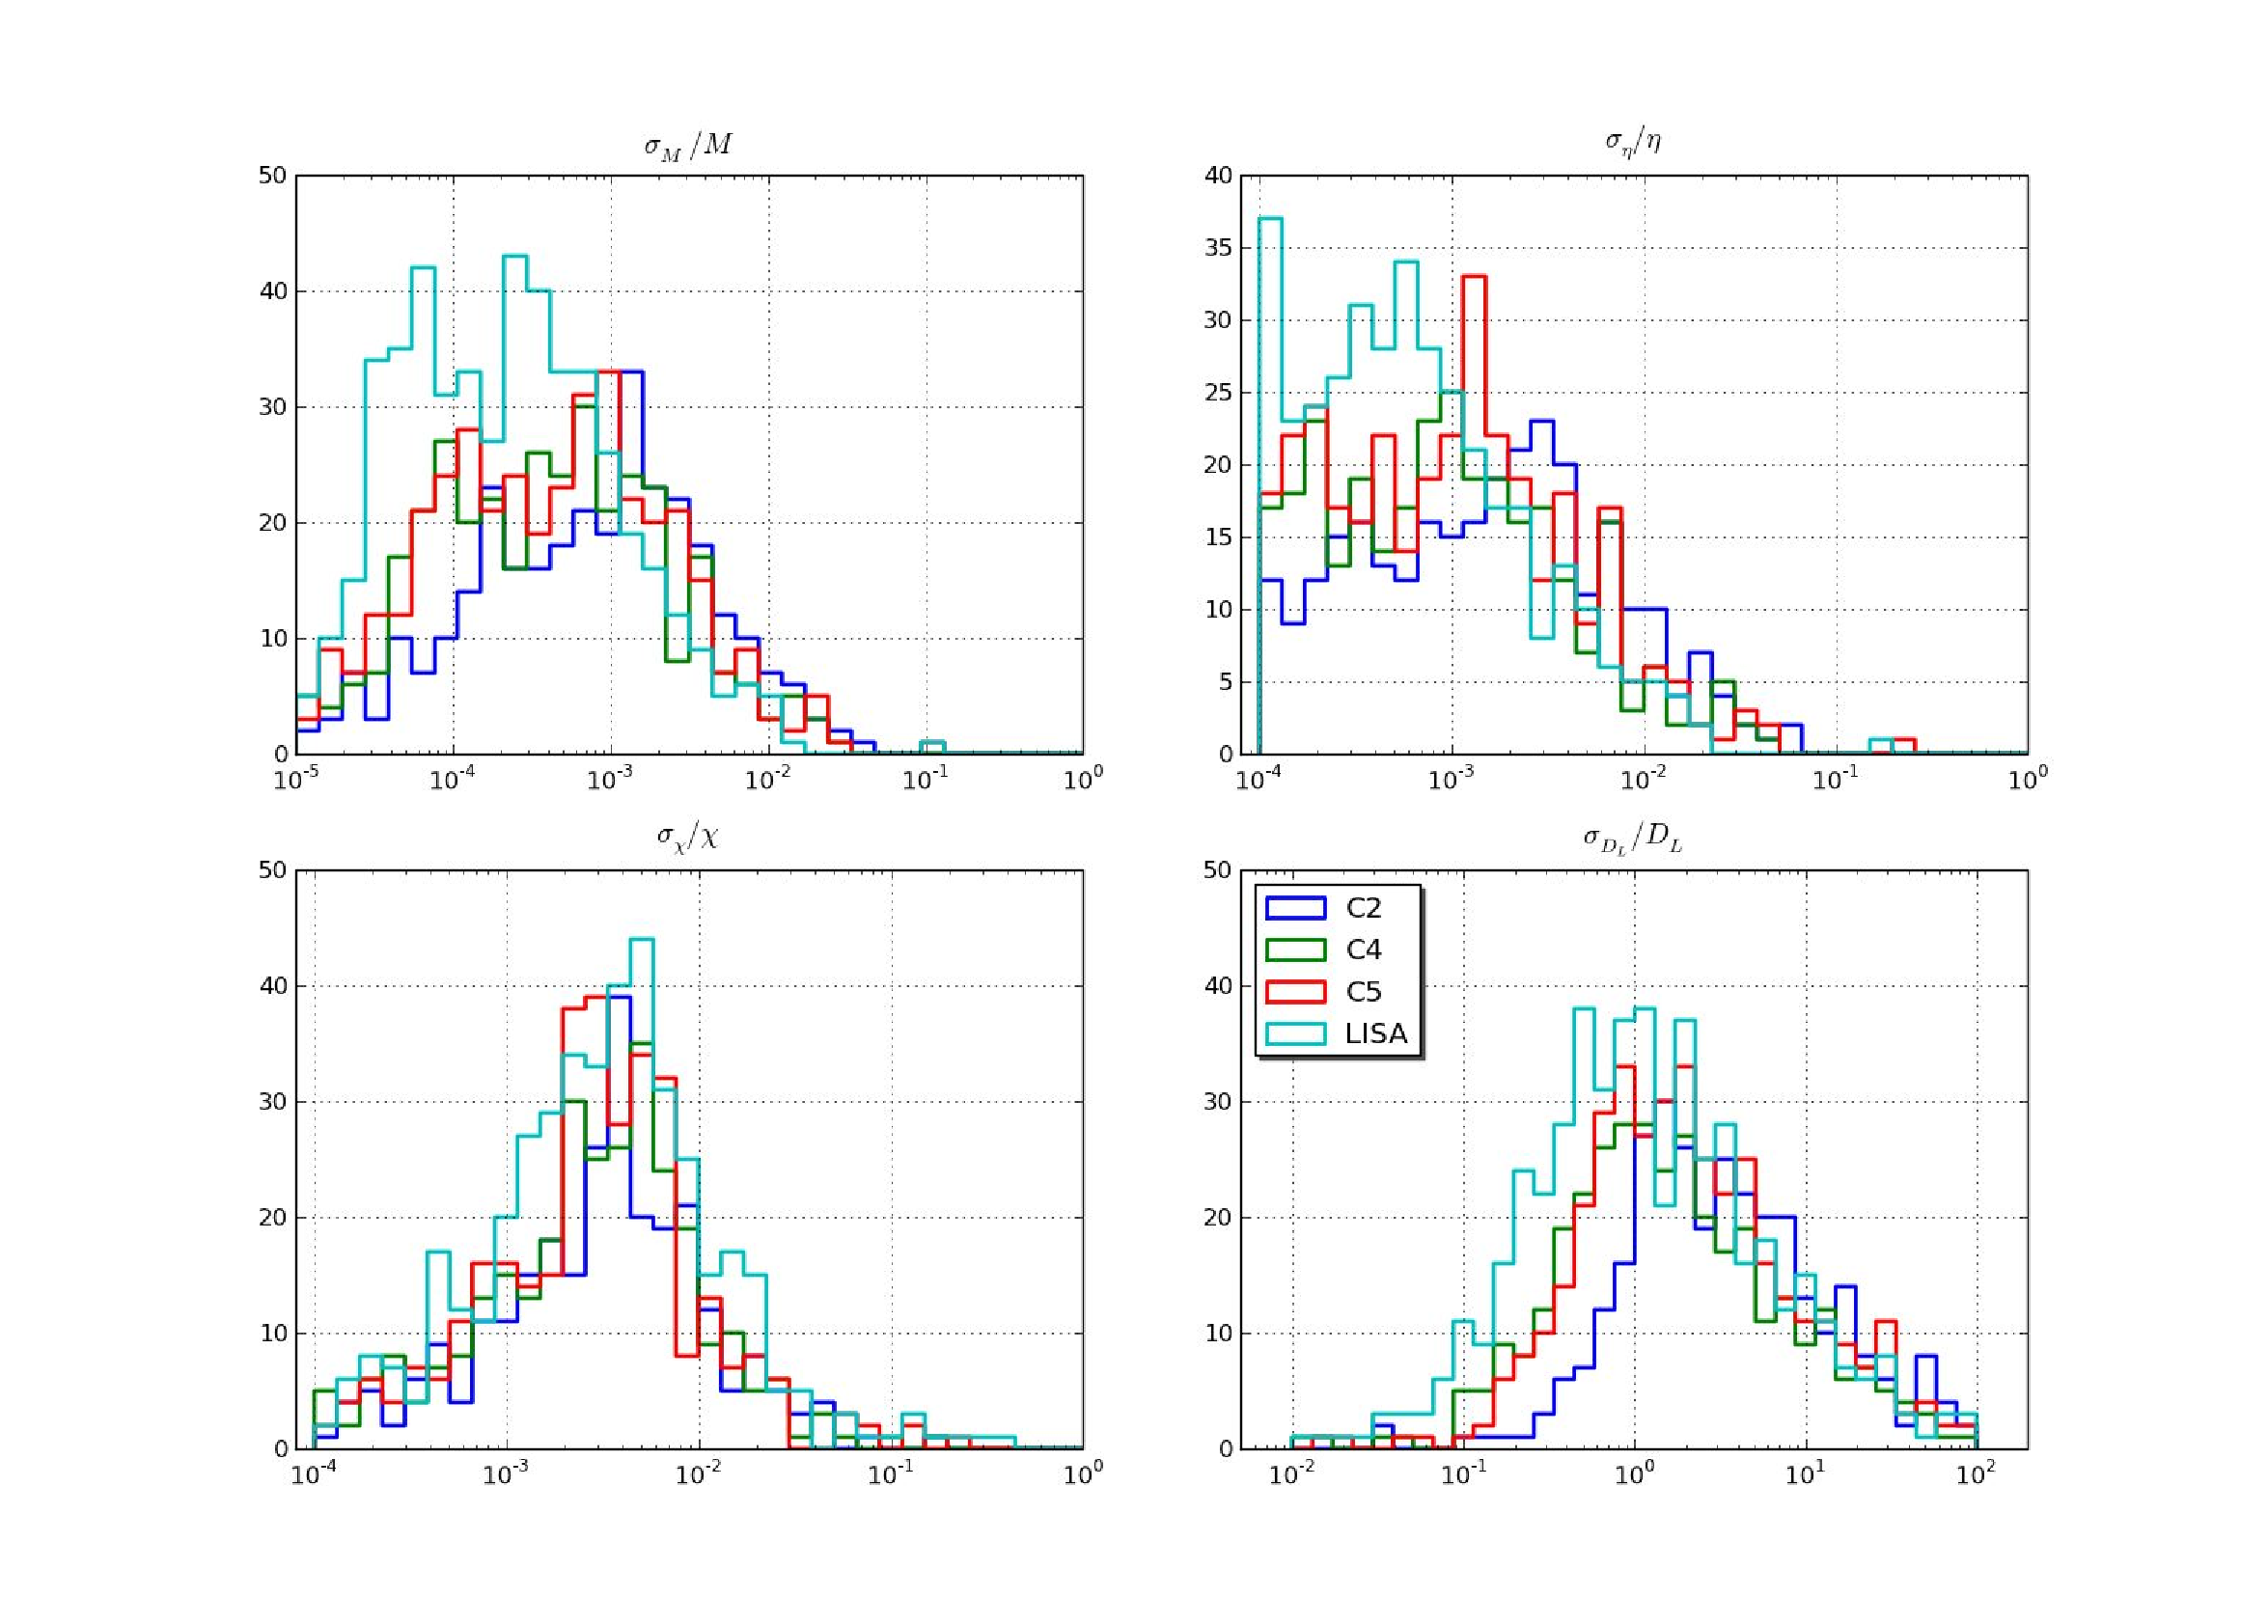
\includegraphics[scale=1,clip]{FigSMBHPhenomAEI/Hist_SE_LISAC2C4C5.eps}} 
\caption{1-$\sigma$ errors on source parameters: redshifted mass (upper left); symmetric mass ratio (upper right); spin parameter (lower left); luminosity distance (lower right). Histograms collect all the events in the SE catalogue (small seed), with SNR$>10$. Ligth blue histograms are for LISA, blue histograms are for C2, green histograms are for C4 and red histograms are for C5.
\label{Hist_SE_LISAC2C4C5} } 
\end{figure}

\begin{figure}
\resizebox{\hsize}{!}{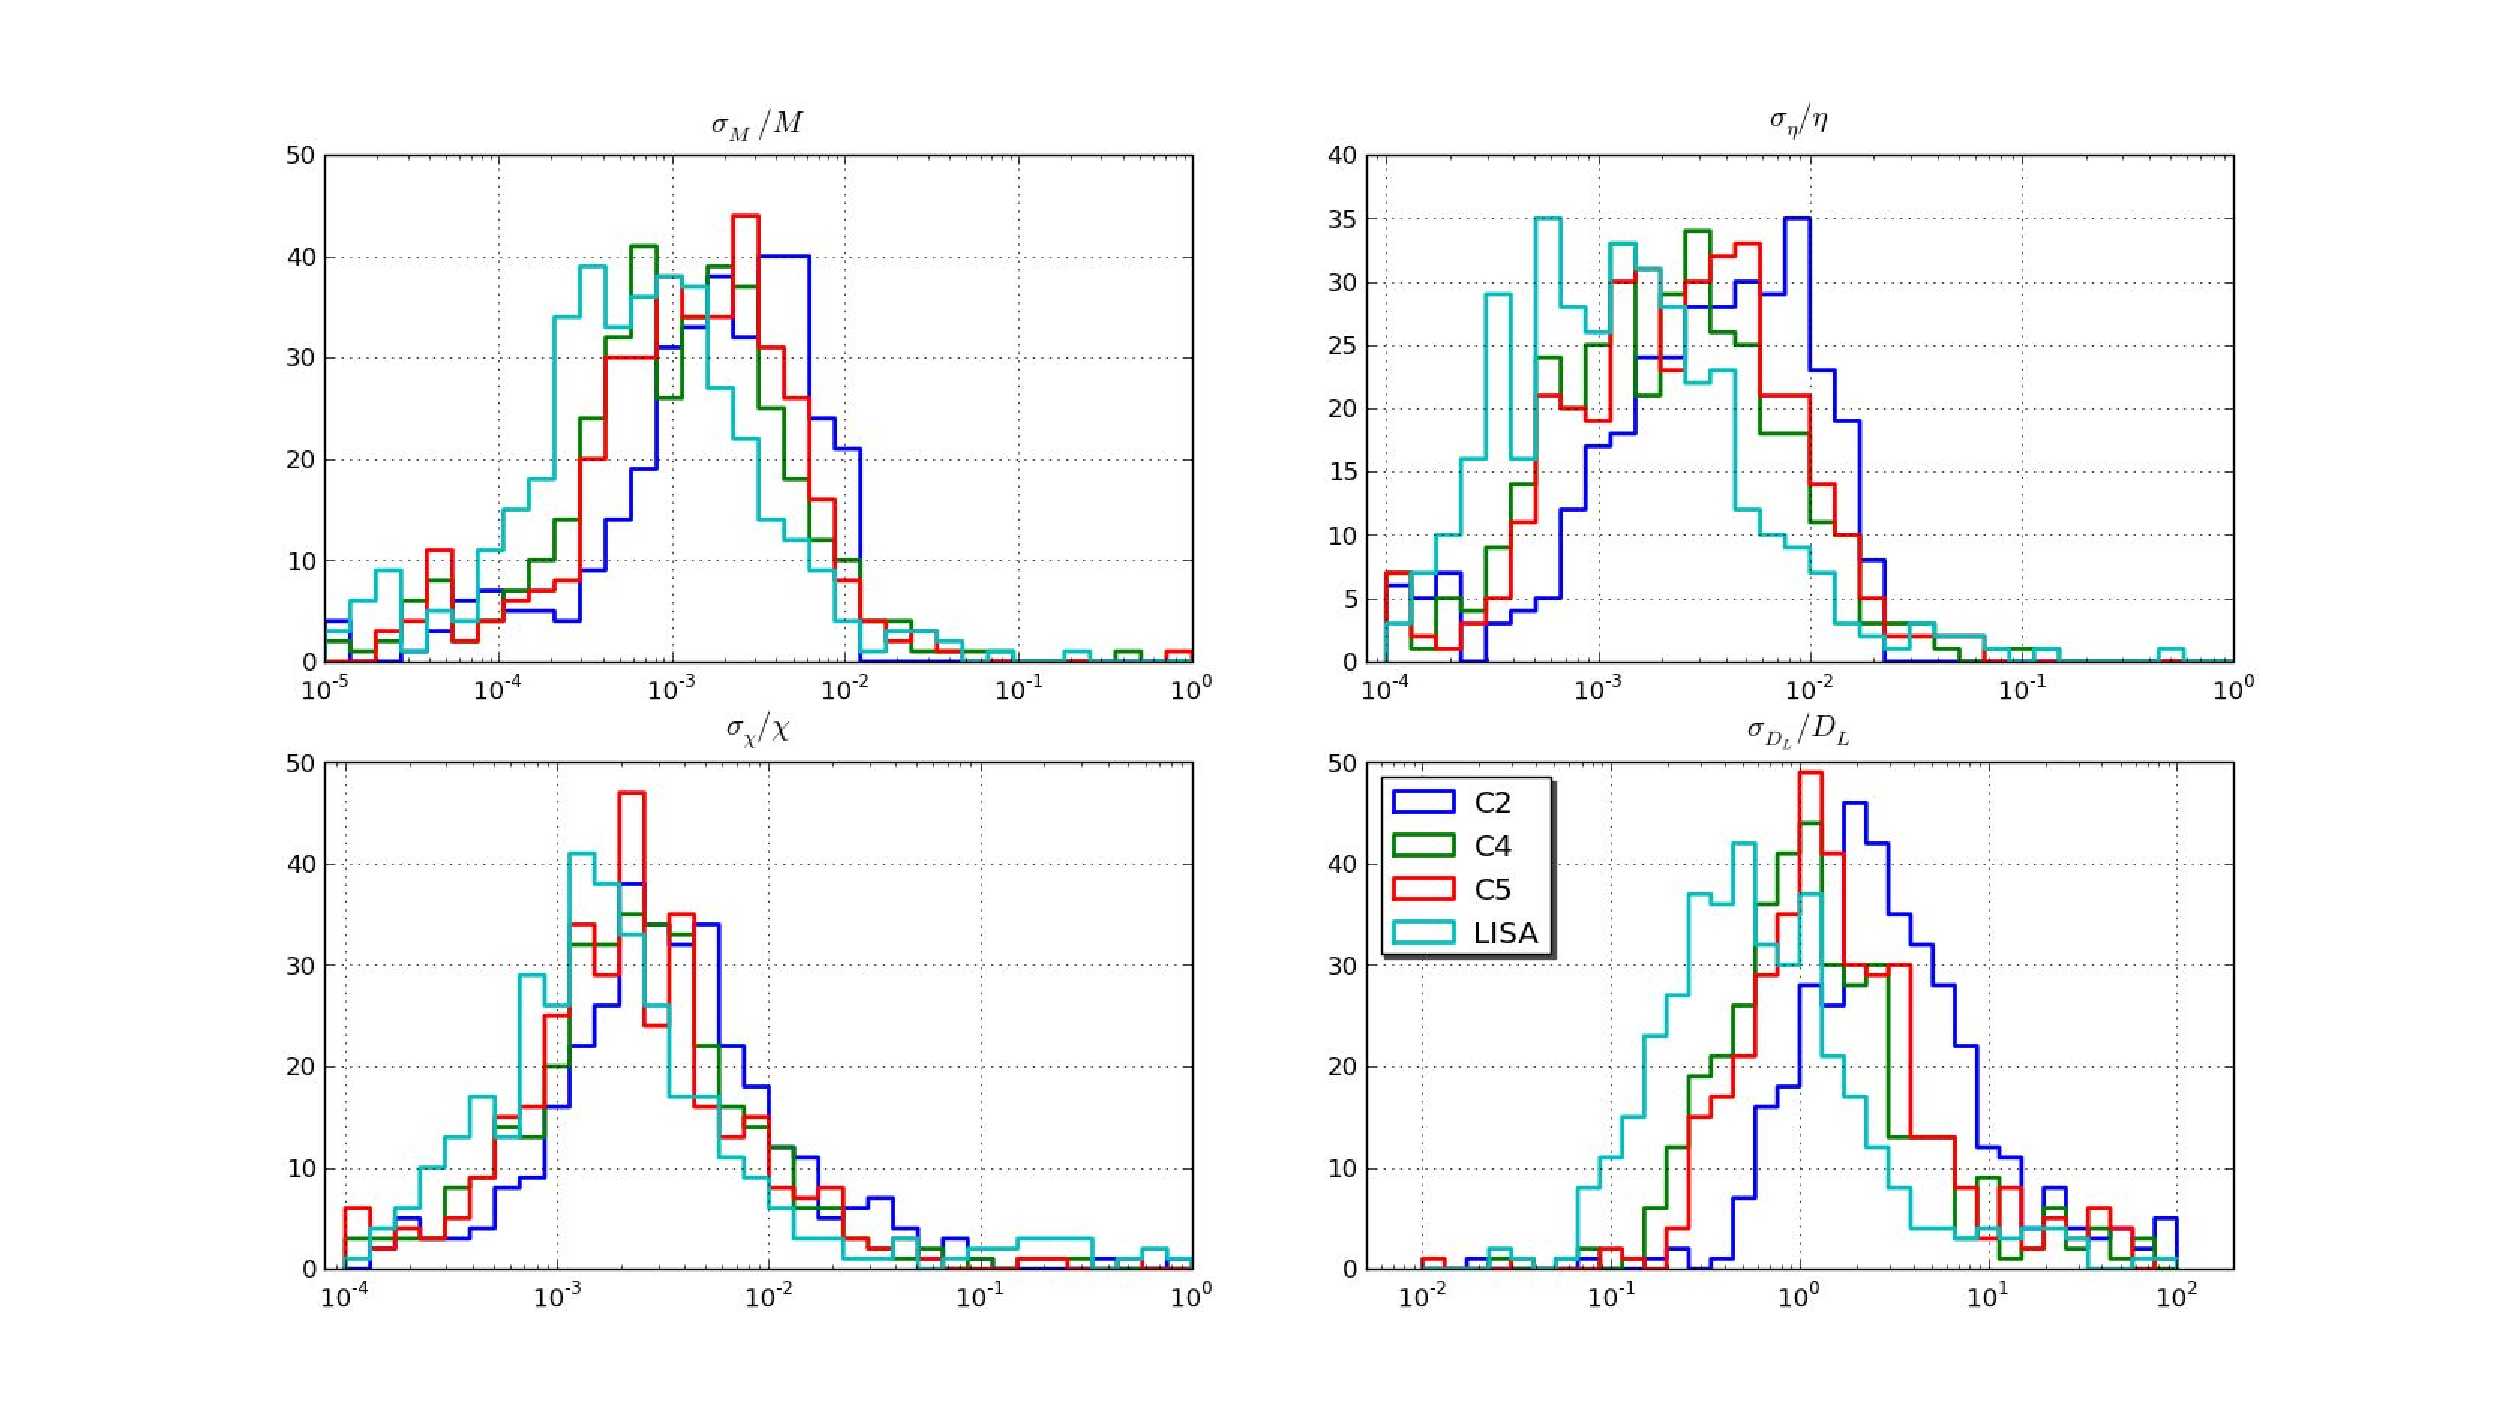
\includegraphics[scale=1,clip]{FigSMBHPhenomAEI/Hist_LE_LISAC2C4C5.eps}} 
\caption{1-$\sigma$ errors on source parameters. Similar as \ref{Hist_SE_LISAC2C4C5} with LE catalogue (large seed).
\label{Hist_LE_LISAC2C4C5} } 
\end{figure}


%%%%%%%%%%%%%%%%  Median errors LISA, C2, C4 and C5  %%%%%%%%%%%%%%%%

\begin{figure}
\resizebox{0.99\hsize}{!}{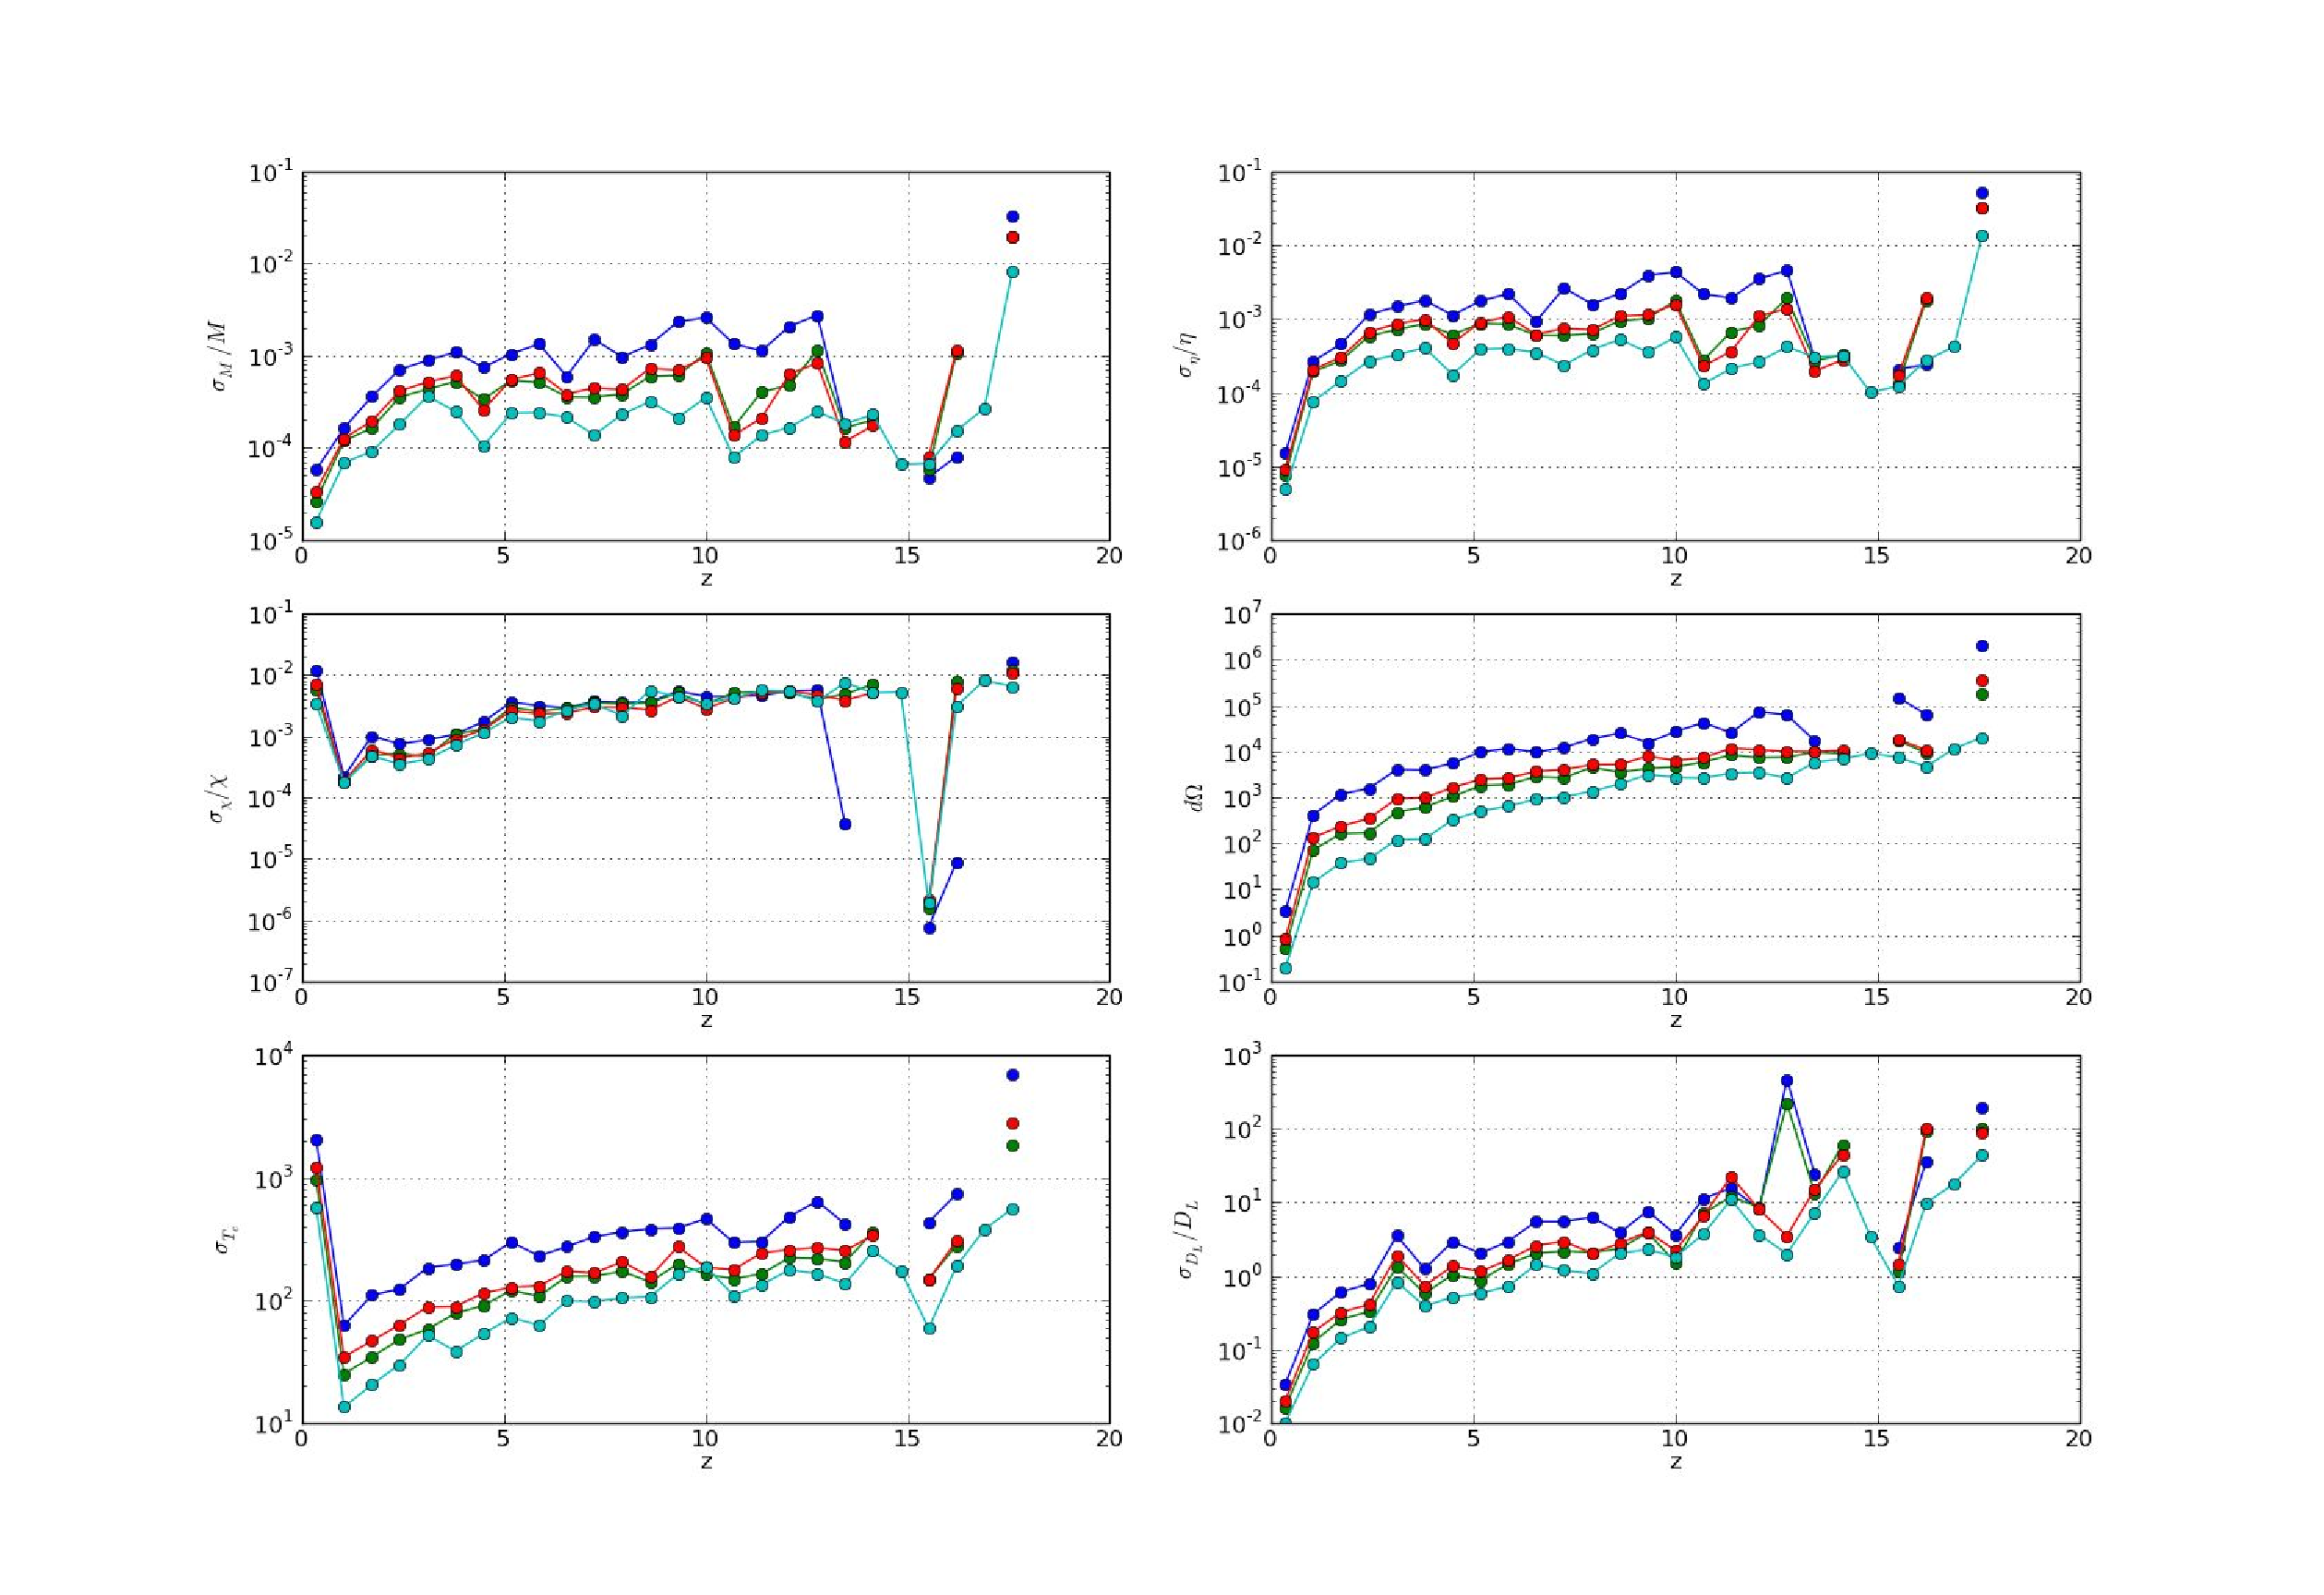
\includegraphics[scale=1,clip]{FigSMBHPhenomAEI/MedianErrs_SE_LISAC2C4C5.eps}} 
\caption{Median 1-$\sigma$ errors on the source parameters as a function of 
$z$: redshifted mass (upper left); symmetric mass ratio (upper right); spin parameter (middle left); sky location in deg$^2$ (middle right); coalescence time in seconds (lower left); luminosity distance (lower right). Colorstyle as in figure \ref{Hist_SE_LISAC2C4C5} : ligth blue histograms are for LISA, blue histograms are for C2, green histograms are for C4 and red histograms are for C5. Model SE (small seeds) is assumed.
\label{MedianErrs_SE_LISAC2C4C5} } 
\end{figure}

\begin{figure}
\resizebox{0.99\hsize}{!}{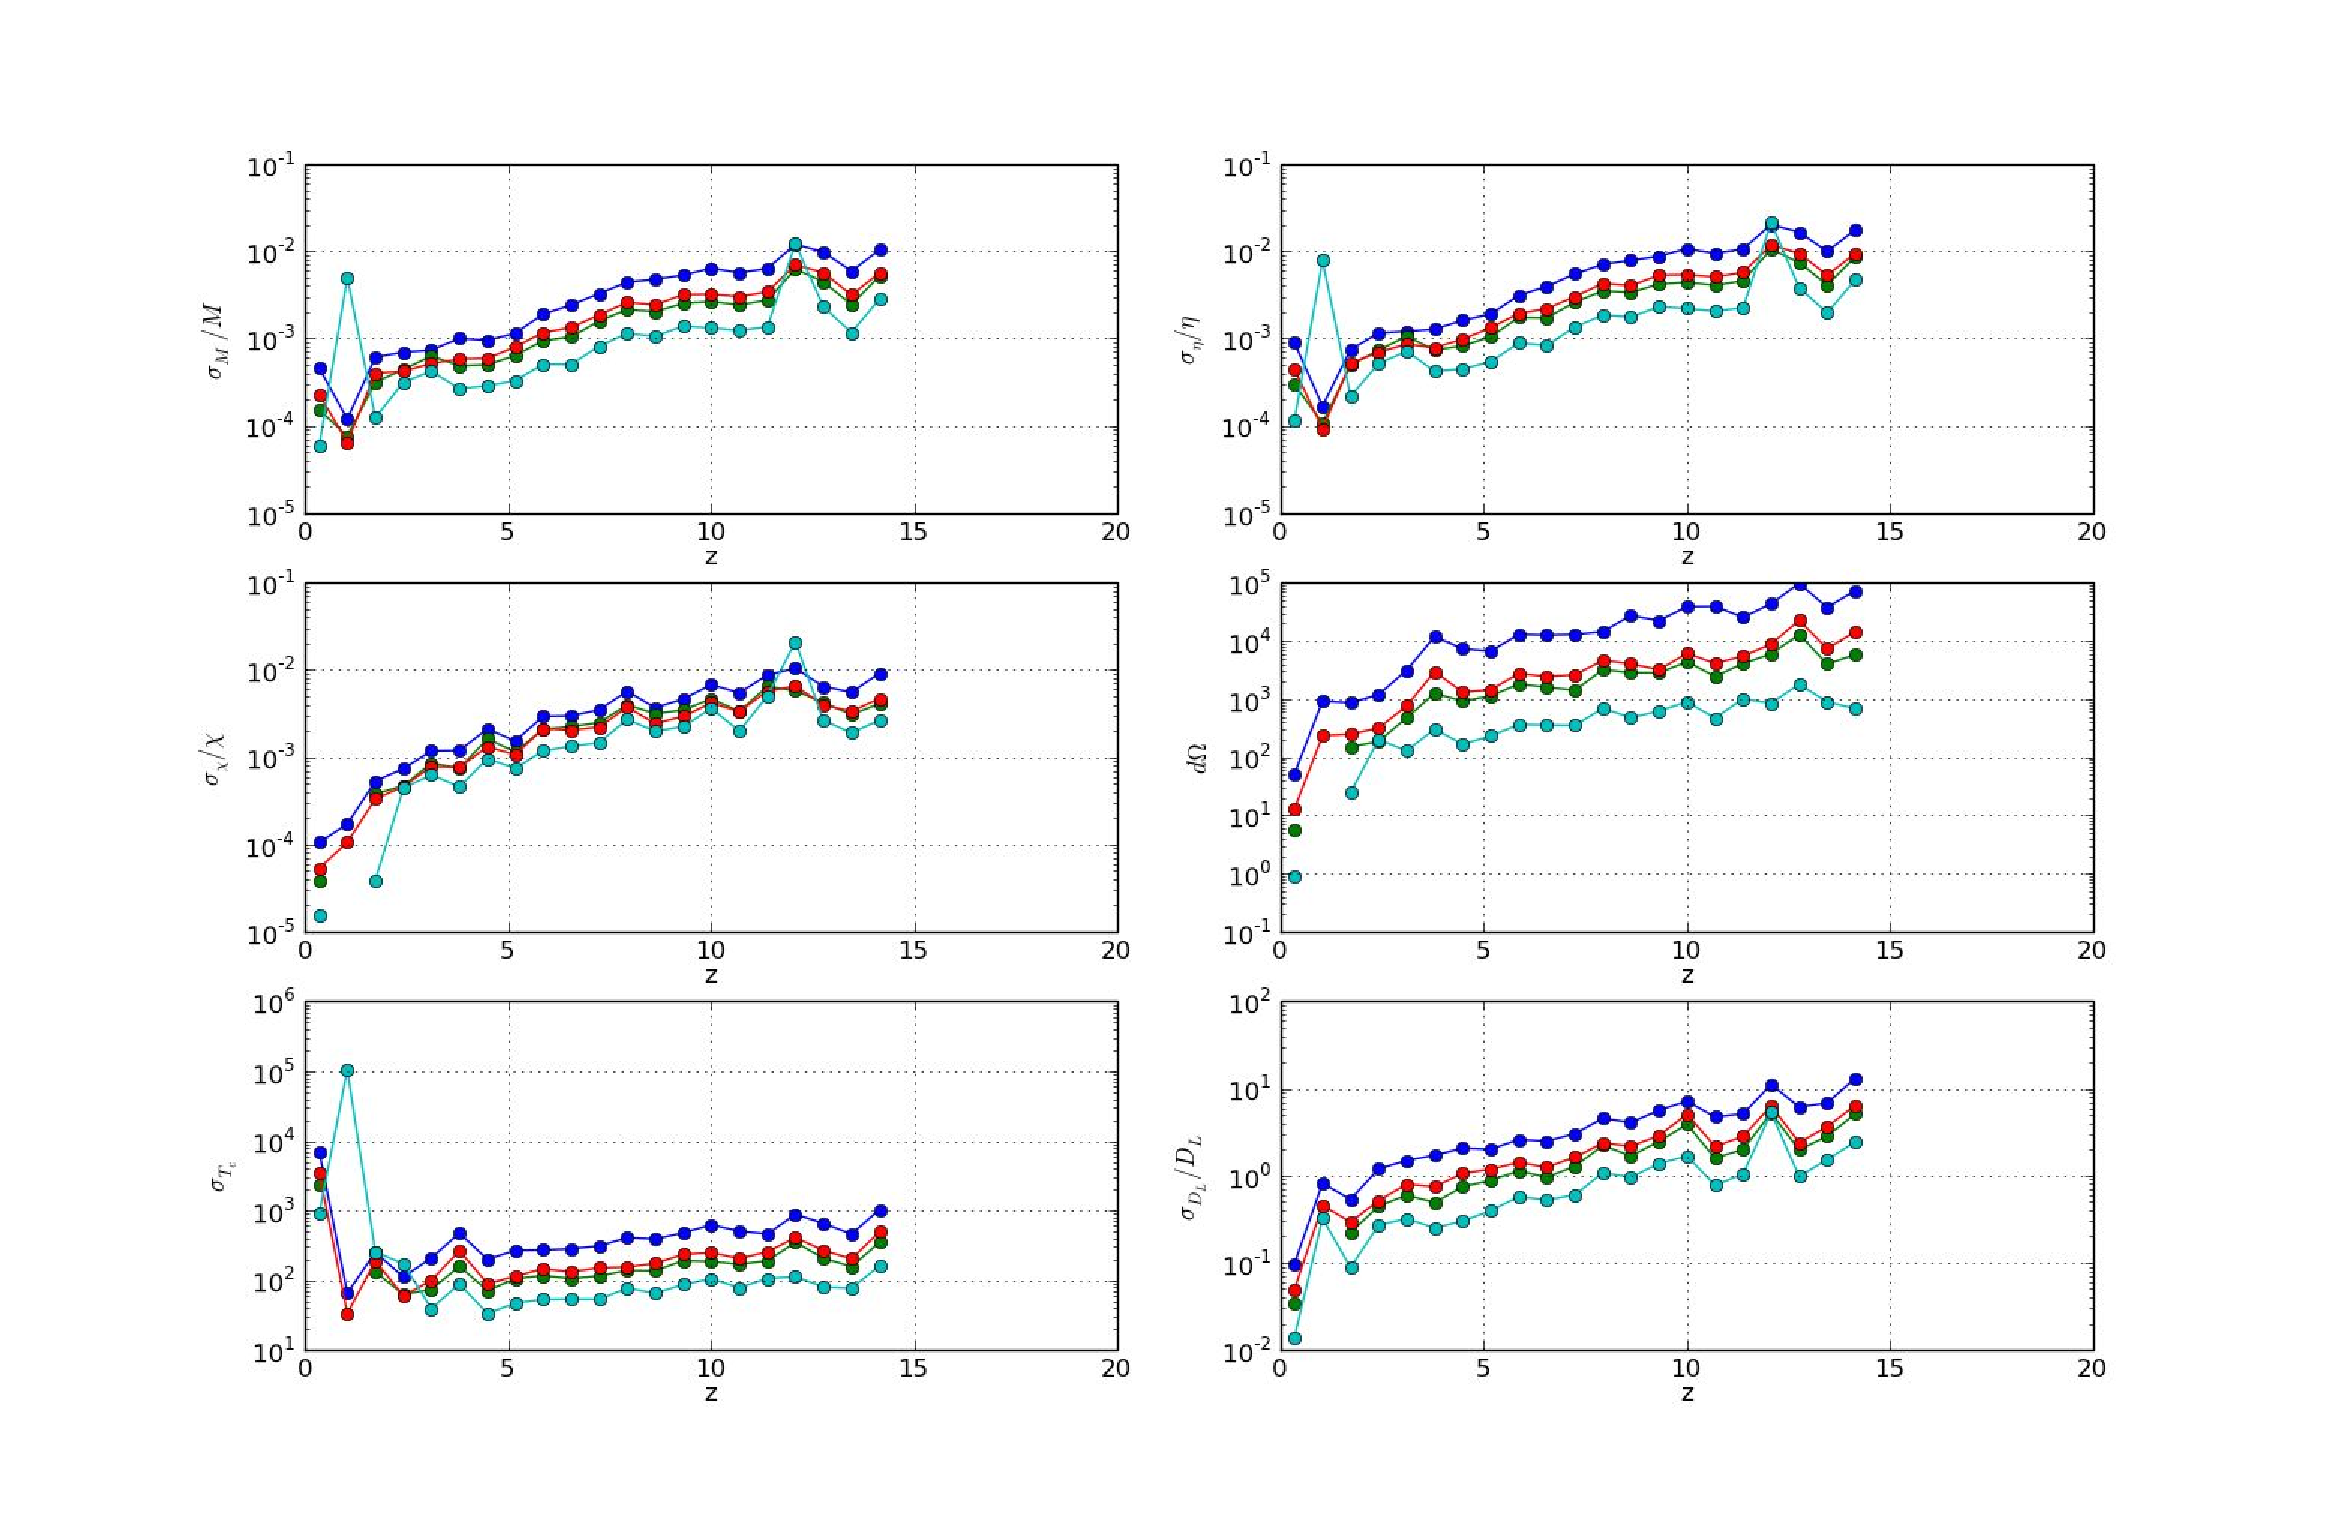
\includegraphics[scale=1,clip]{FigSMBHPhenomAEI/MedianErrs_LE_LISAC2C4C5.eps}} 
\caption{Same as figure \ref{MedianErrs_SE_LISAC2C4C5} but for the LE (large seed) catalogue.
\label{MedianErrs_LE_LISAC2C4C5} } 
\end{figure}


%%%%%%%%%%%%%%%%  Median SNR LISA, C2, C4 and C5  %%%%%%%%%%%%%%%%


\begin{figure}
\resizebox{0.95\hsize}{!}{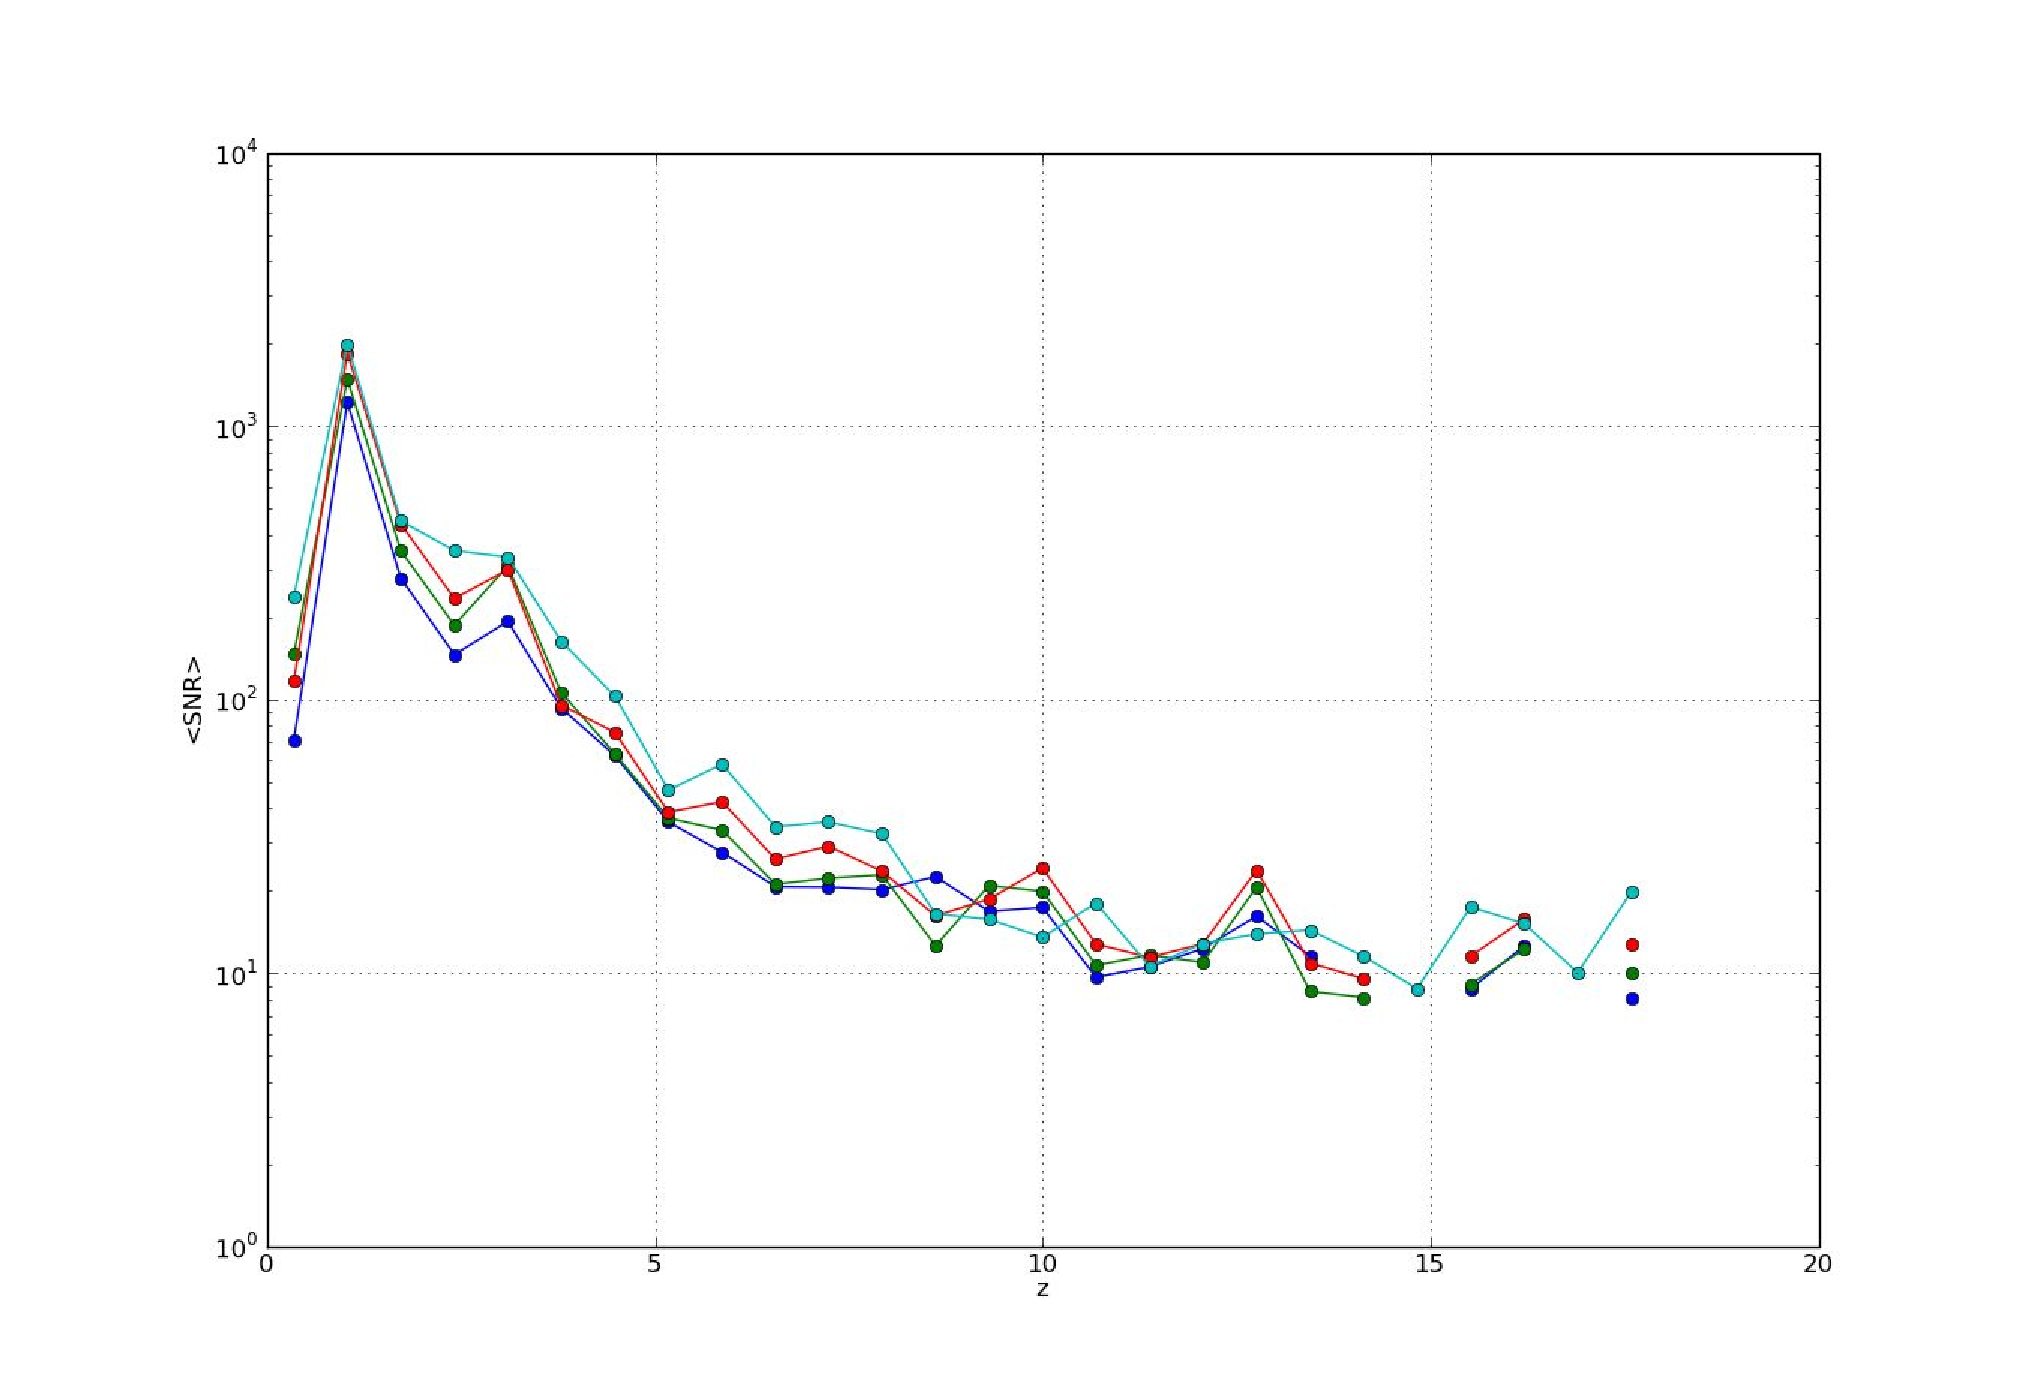
\includegraphics[scale=1,clip]{FigSMBHPhenomAEI/MedianSNR_SE_LISAC2C4C5.eps}} 
\caption{Median SNR s as a function of  $z$. Colorstyle as in figure \ref{Hist_SE_LISAC2C4C5} : ligth blue histograms are for LISA, blue histograms are for C2, green histograms are for C4 and red histograms are for C5. Model SE (small seeds) is assumed.
\label{MedianSNR_SE_LISAC2C4C5} } 
\end{figure}

\begin{figure}
\resizebox{0.95\hsize}{!}{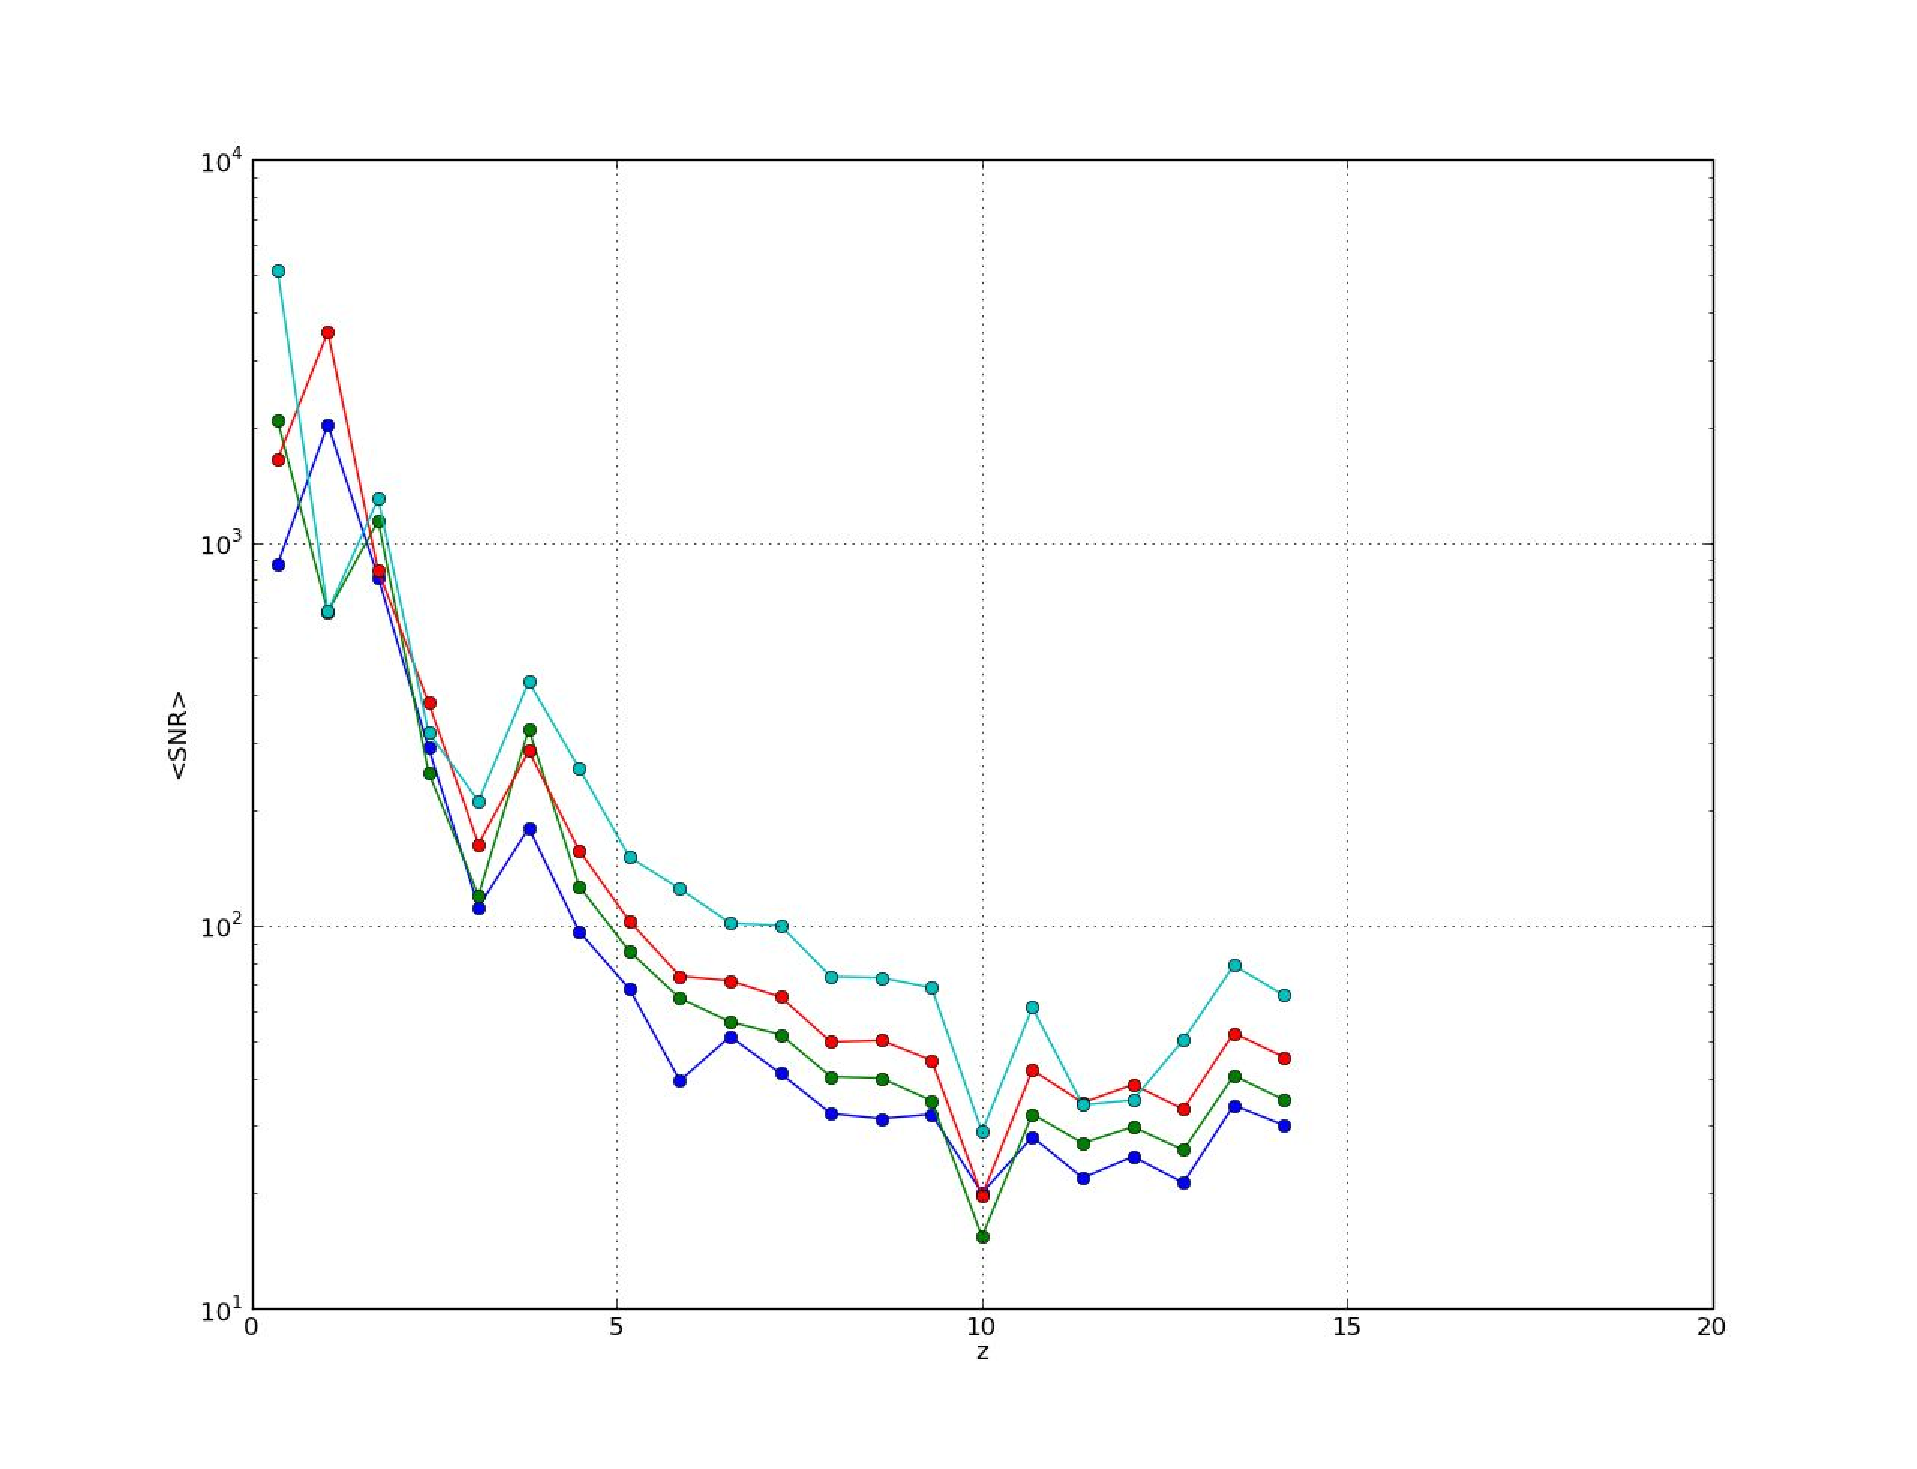
\includegraphics[scale=1,clip]{FigSMBHPhenomAEI/MedianSNR_LE_LISAC2C4C5.eps}} 
\caption{Same as figure \ref{MedianSNR_SE_LISAC2C4C5} but for the LE (large seed) catalogue.
\label{MedianSNR_LE_LISAC2C4C5} } 
\end{figure}


%%%%%%%%%%%%%%%%  SNR vs z LISA, C1 and C3  %%%%%%%%%%%%%%%%


\begin{figure}
\resizebox{\hsize}{!}{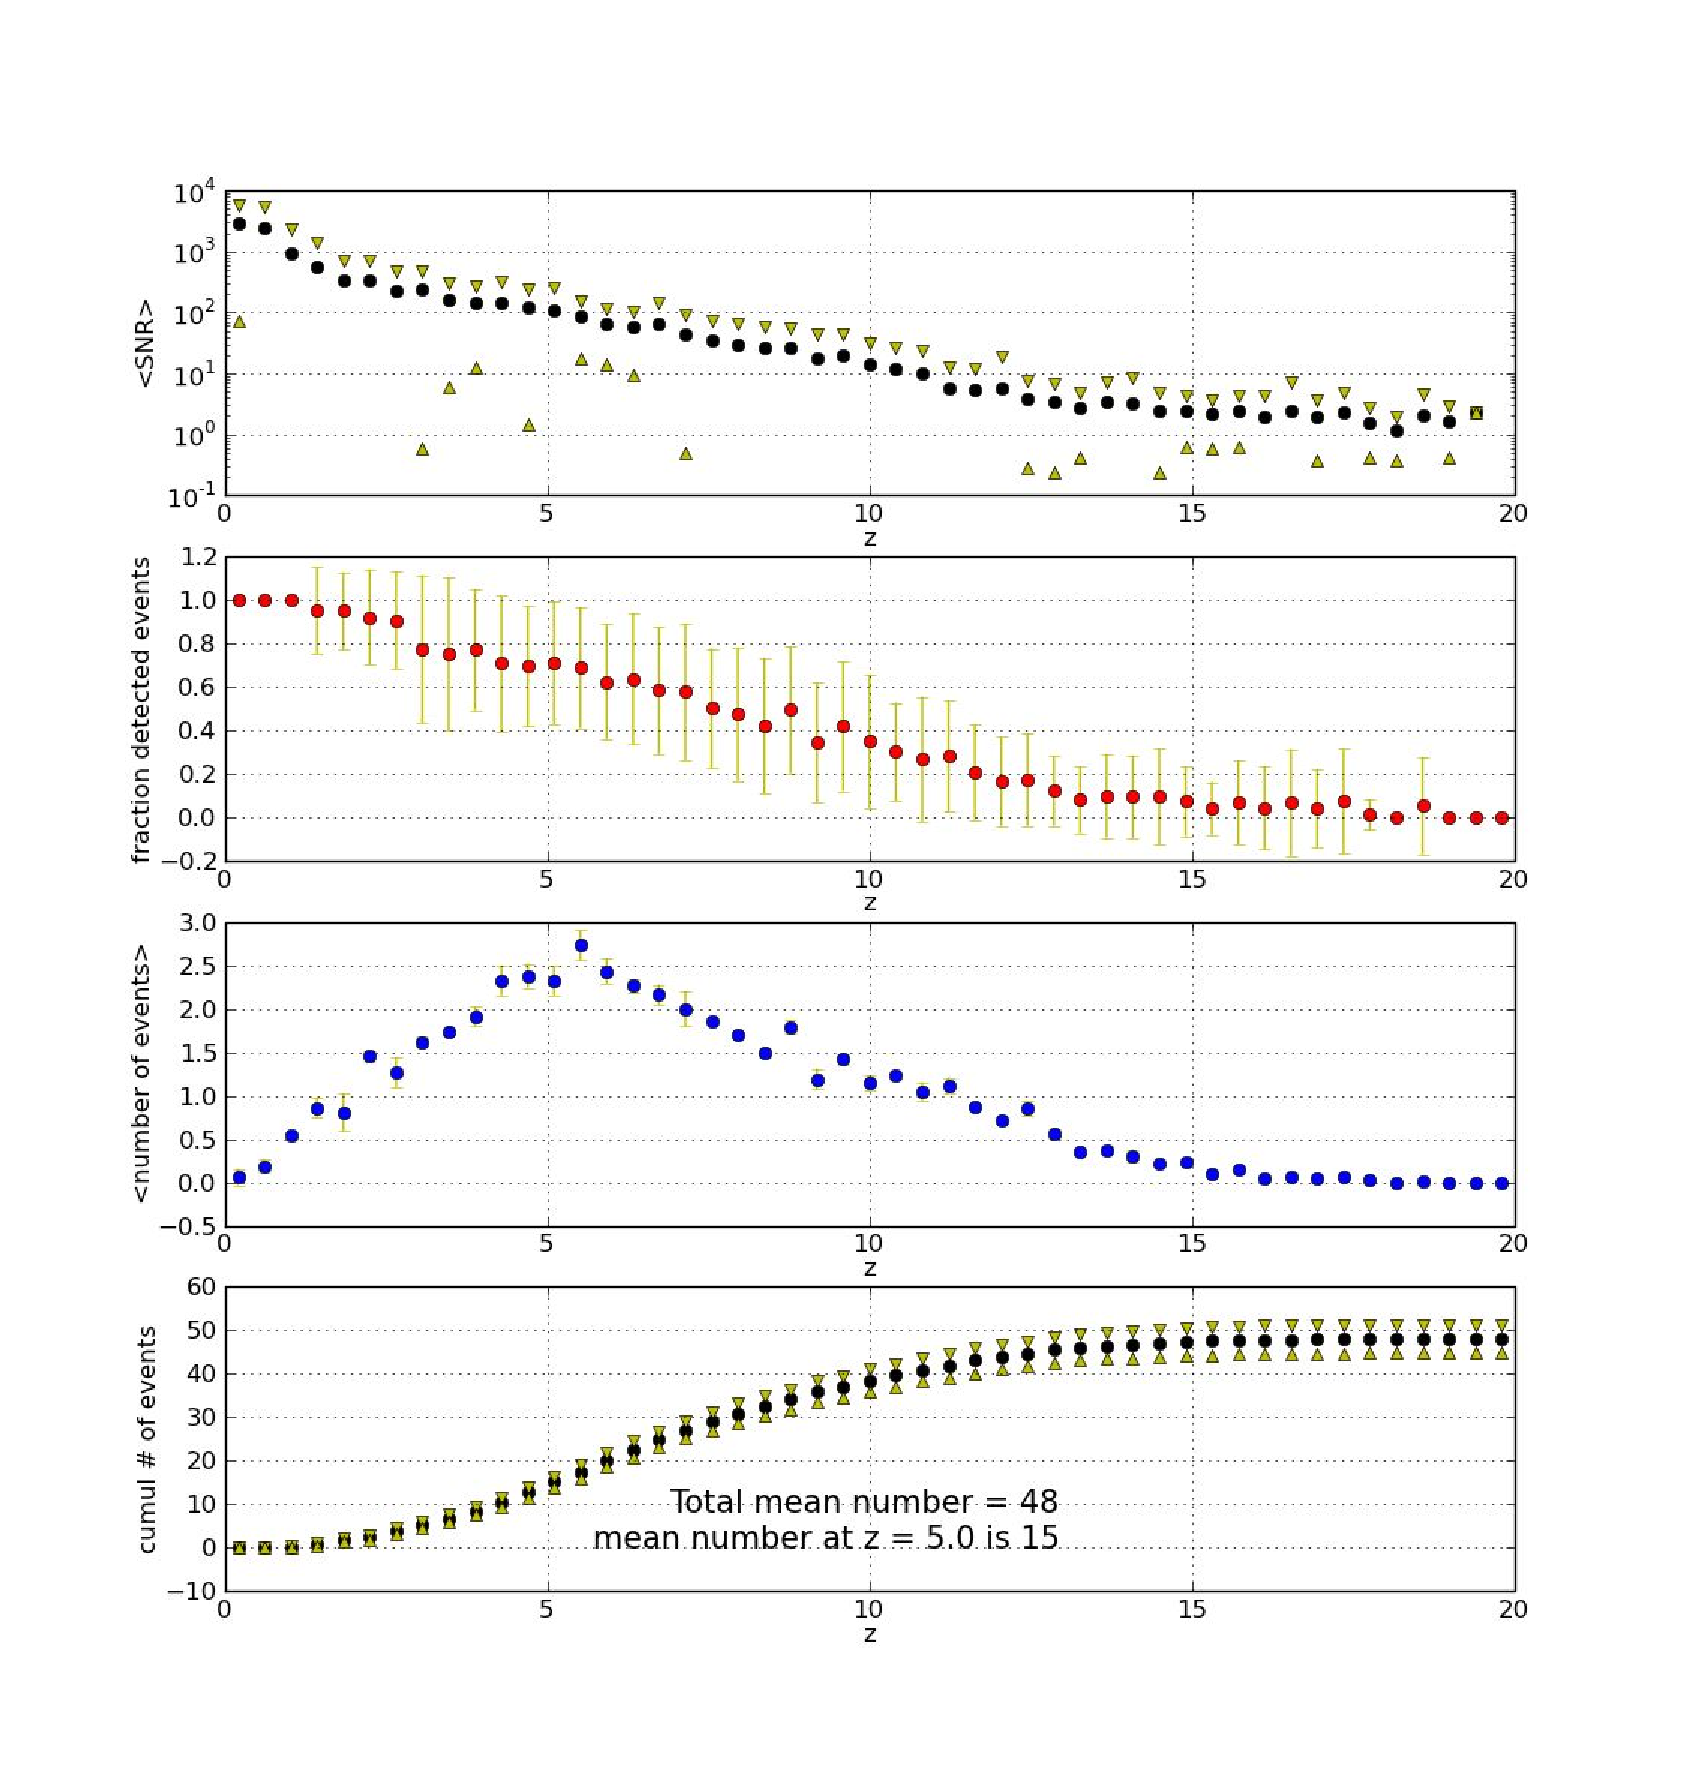
\includegraphics[scale=1,clip]{FigSMBHPhenomAEI/LISA_mc_SNRs.eps}} 
\caption{LISA performances as a function of redshift. From the top to the bottom we plot the average source SNR, the fraction of detectable sources (SNR$>6$), the mean number of detected sources, and the cumulative number of detected sources. Error bars are standard deviations; SE population model is assumed.
\label{LISA_mc_SNR} } 
\end{figure}


\begin{figure}
\resizebox{\hsize}{!}{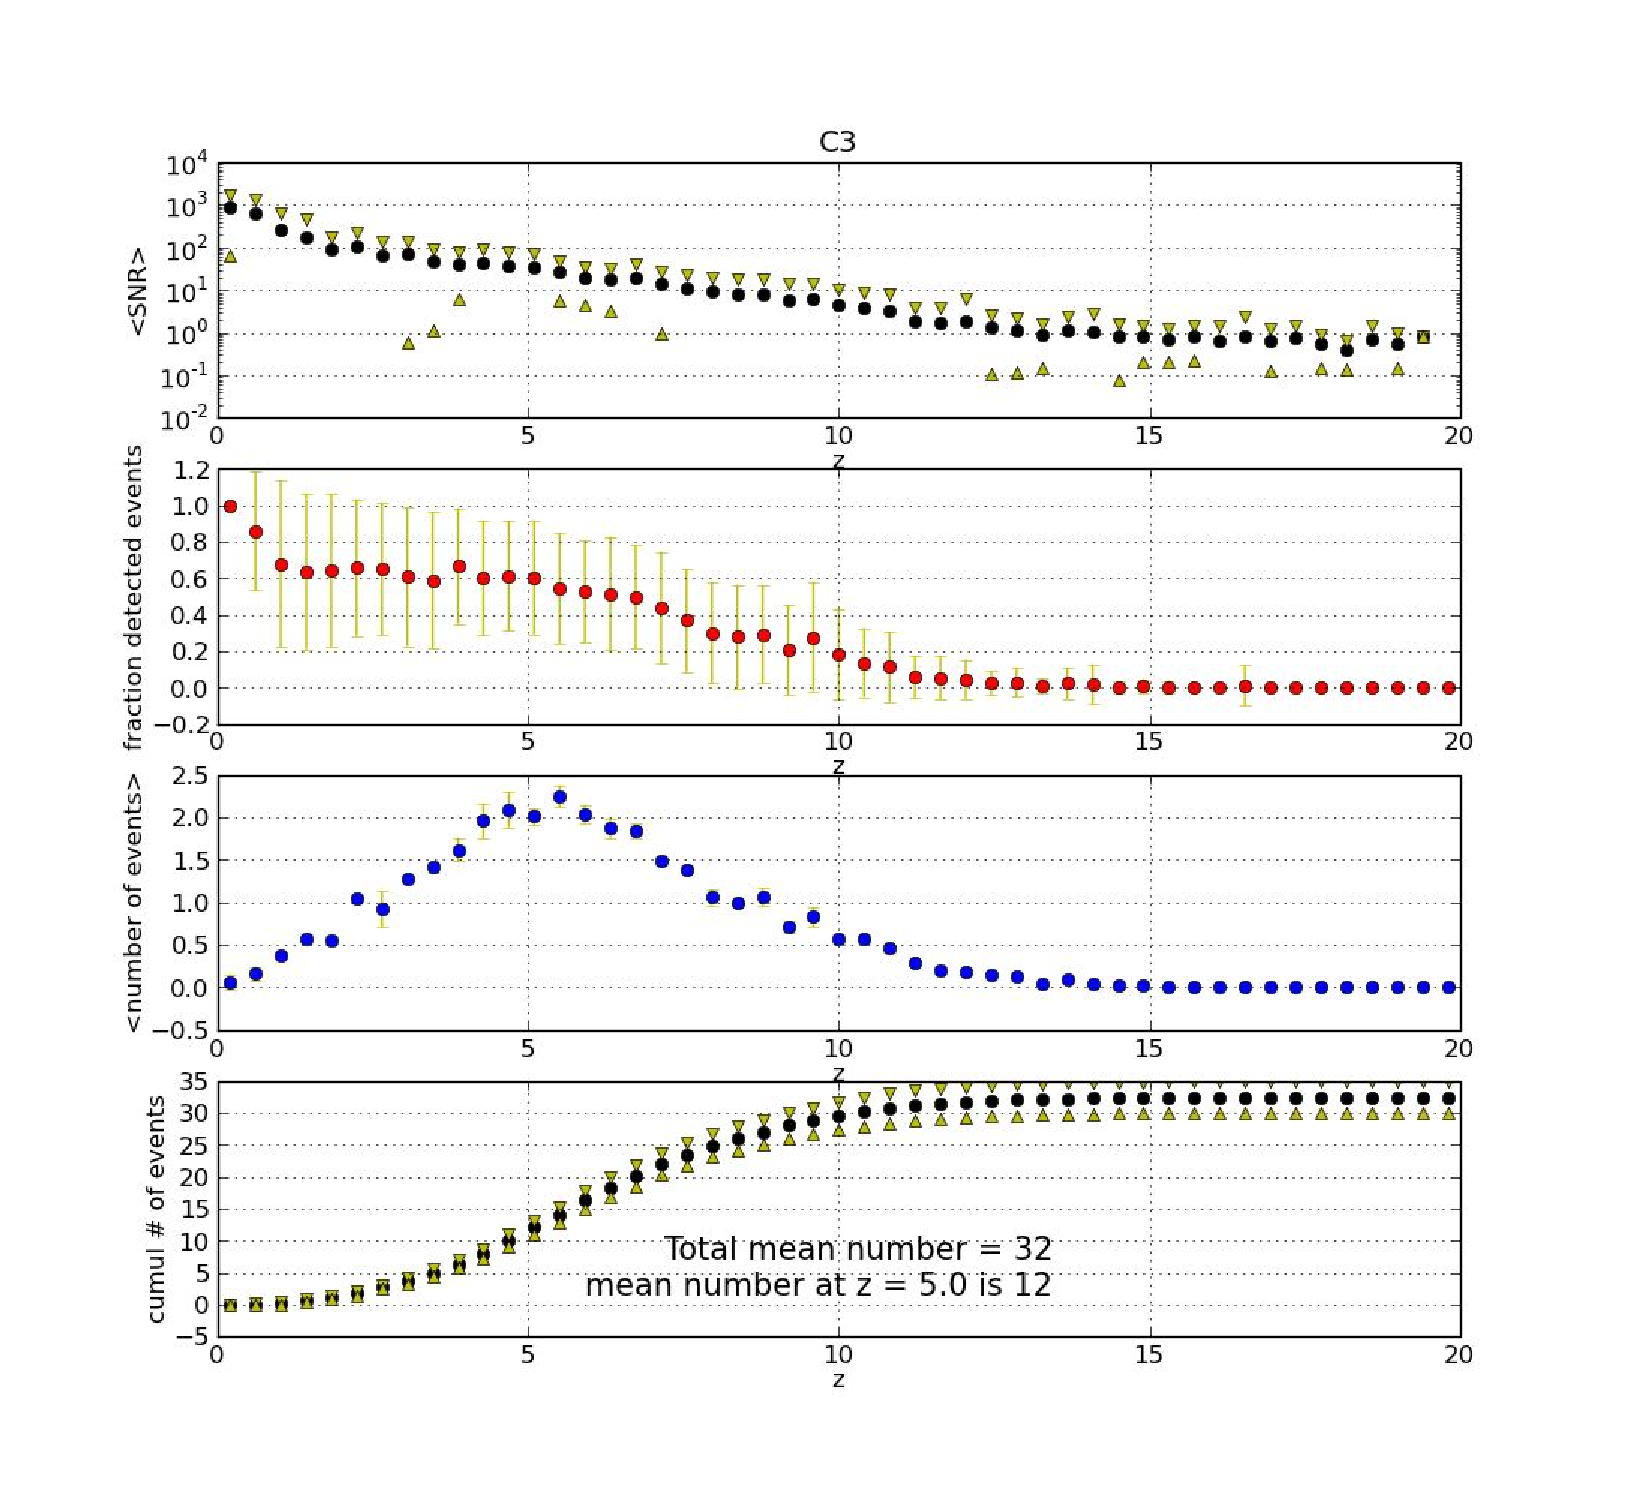
\includegraphics[scale=1,clip]{FigSMBHPhenomAEI/C3_mc_SNRs.eps}} 
\caption{Same as figure \ref{LISA_mc_SNR} but for C3.
\label{C3_mc_SNR} } 
\end{figure}


\begin{figure}
\resizebox{\hsize}{!}{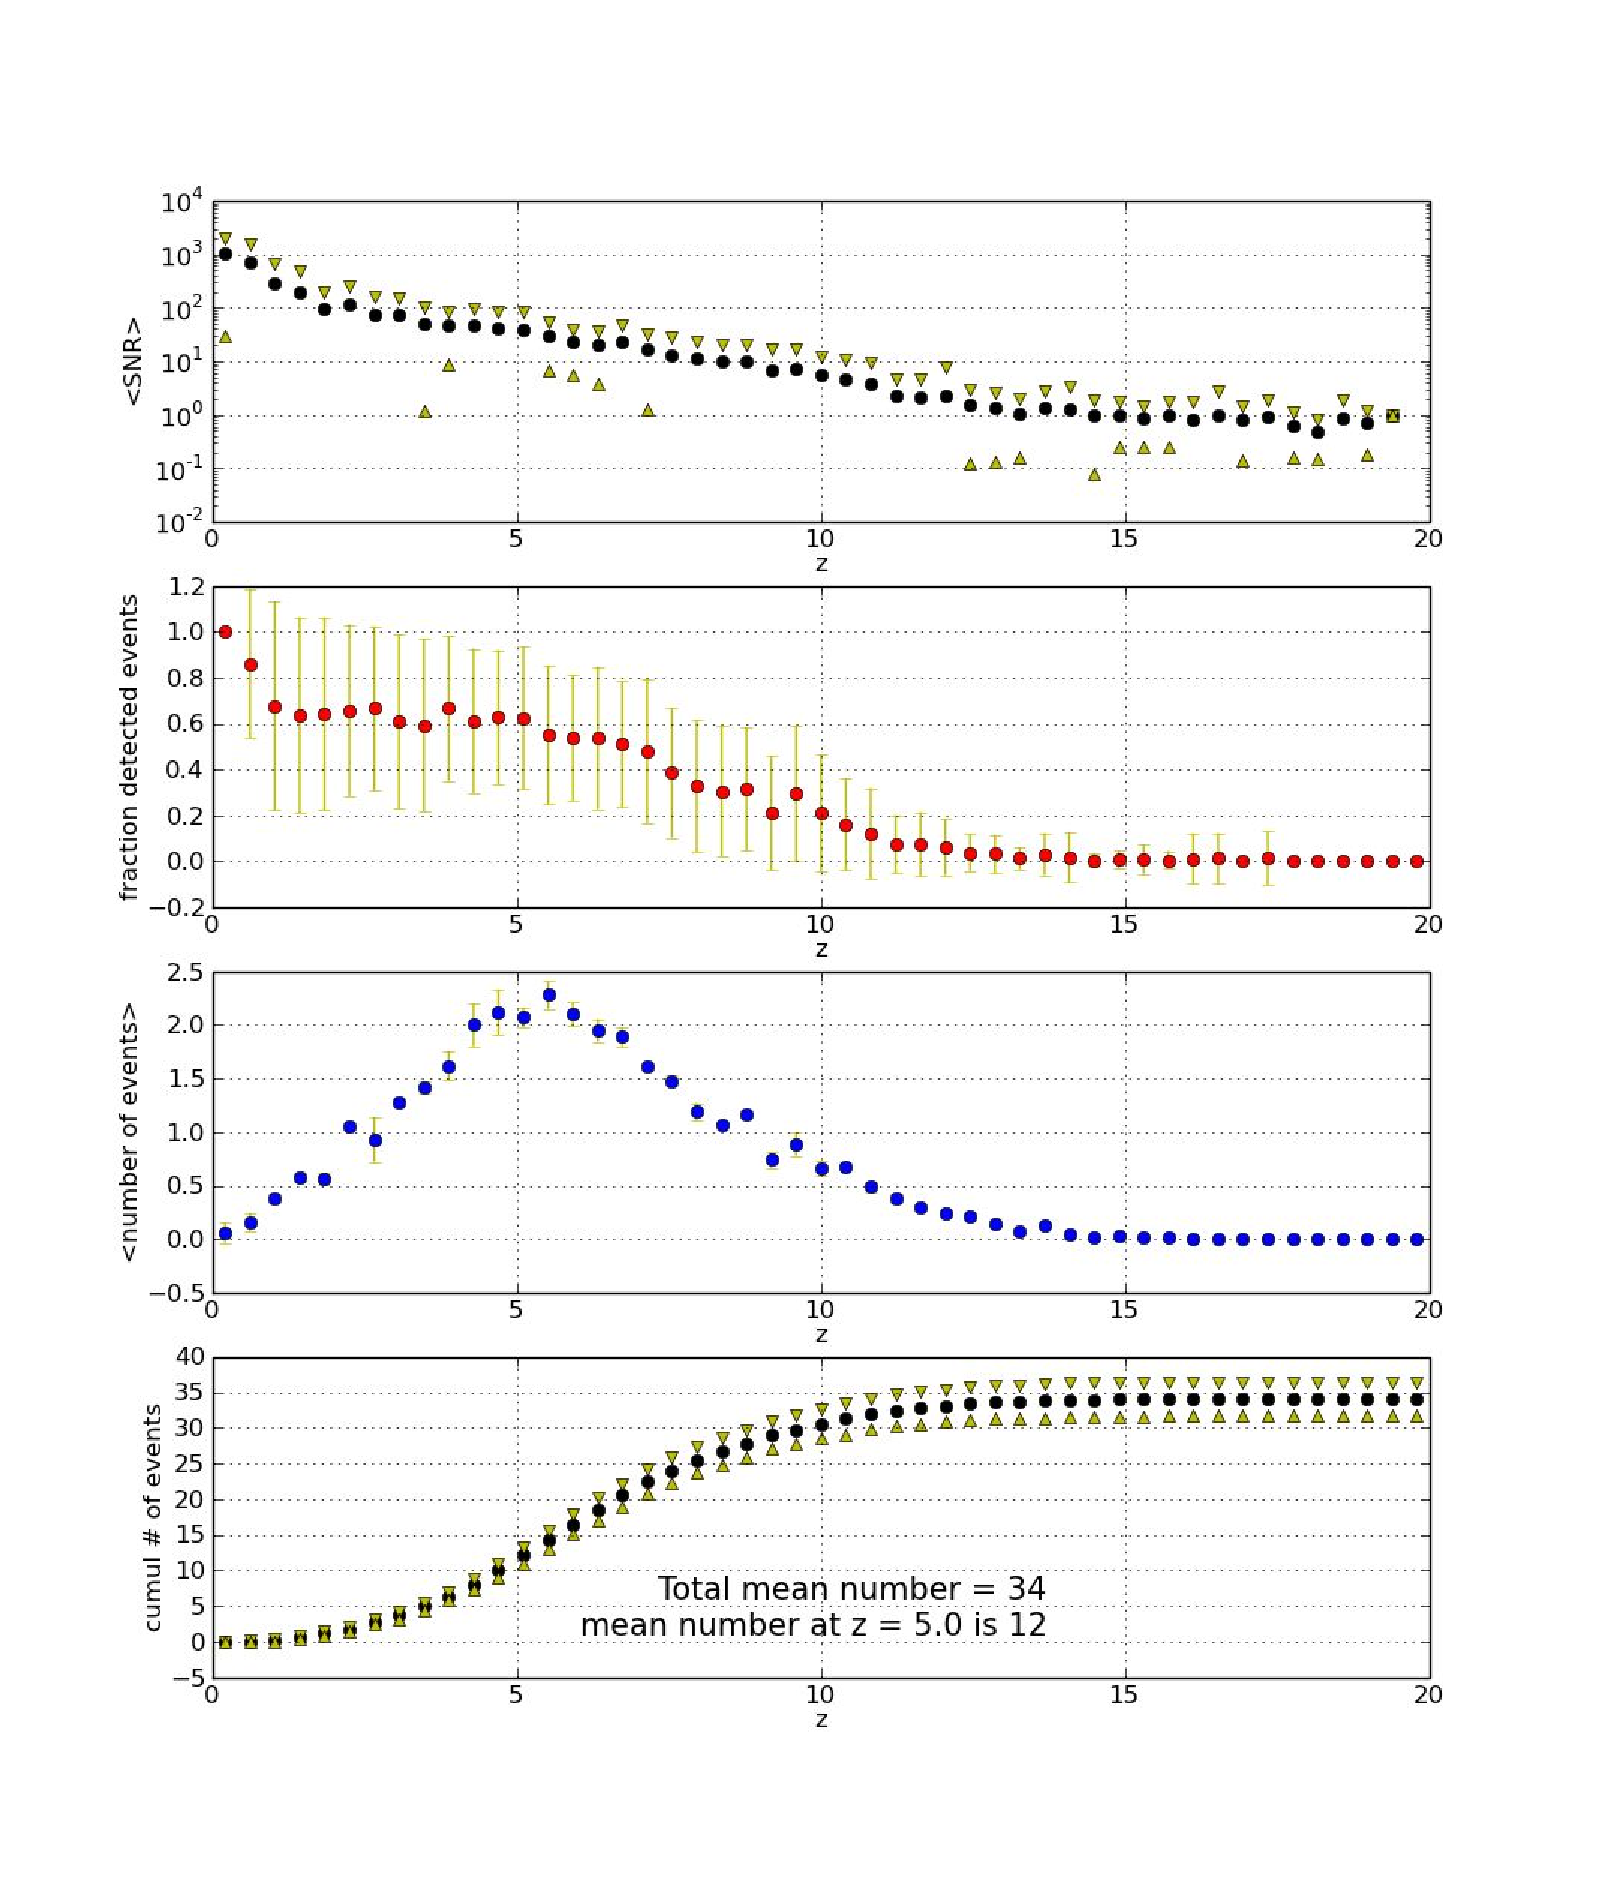
\includegraphics[scale=1,clip]{FigSMBHPhenomAEI/C2_mc_SNRs.eps}} 
\caption{Same as figure \ref{LISA_mc_SNR} but for C2.
\label{C2_mc_SNR} } 
\end{figure}


\begin{figure}
\resizebox{\hsize}{!}{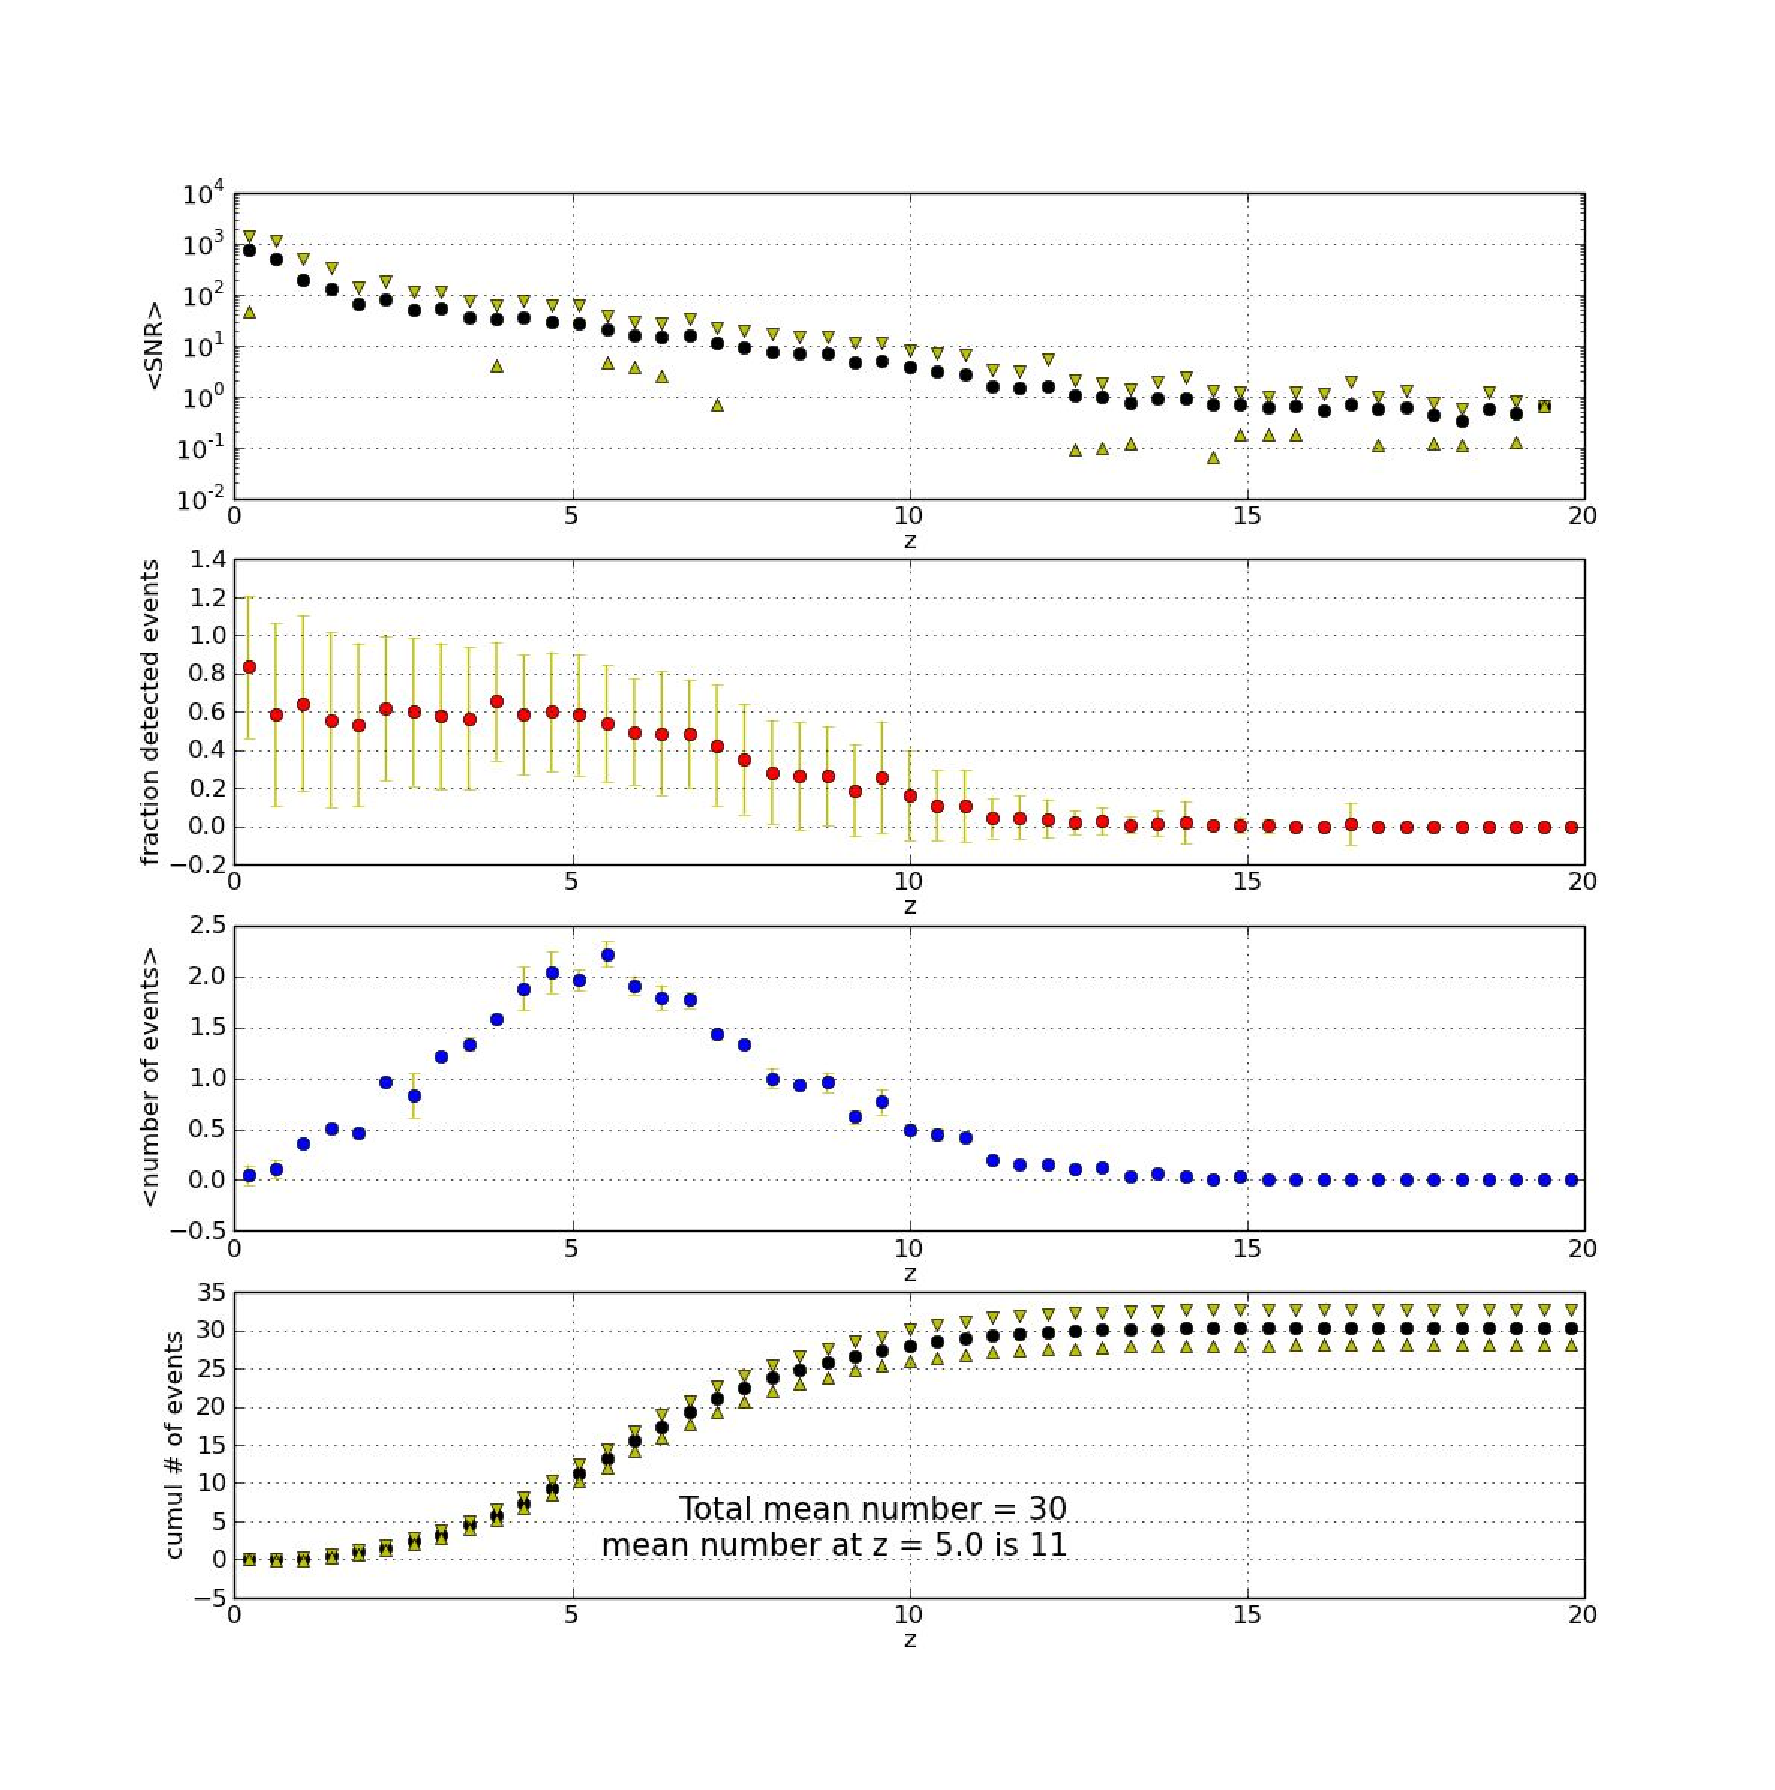
\includegraphics[scale=1,clip]{FigSMBHPhenomAEI/C1_mc_SNRs}} 
\caption{Same as figure \ref{LISA_mc_SNR} but for C1.
\label{C1_mc_SNR} } 
\end{figure}



%%%%%%%%%%%%%%%%  Histogram LISA, C1 and C3  %%%%%%%%%%%%%%%%


\begin{figure}
\resizebox{\hsize}{!}{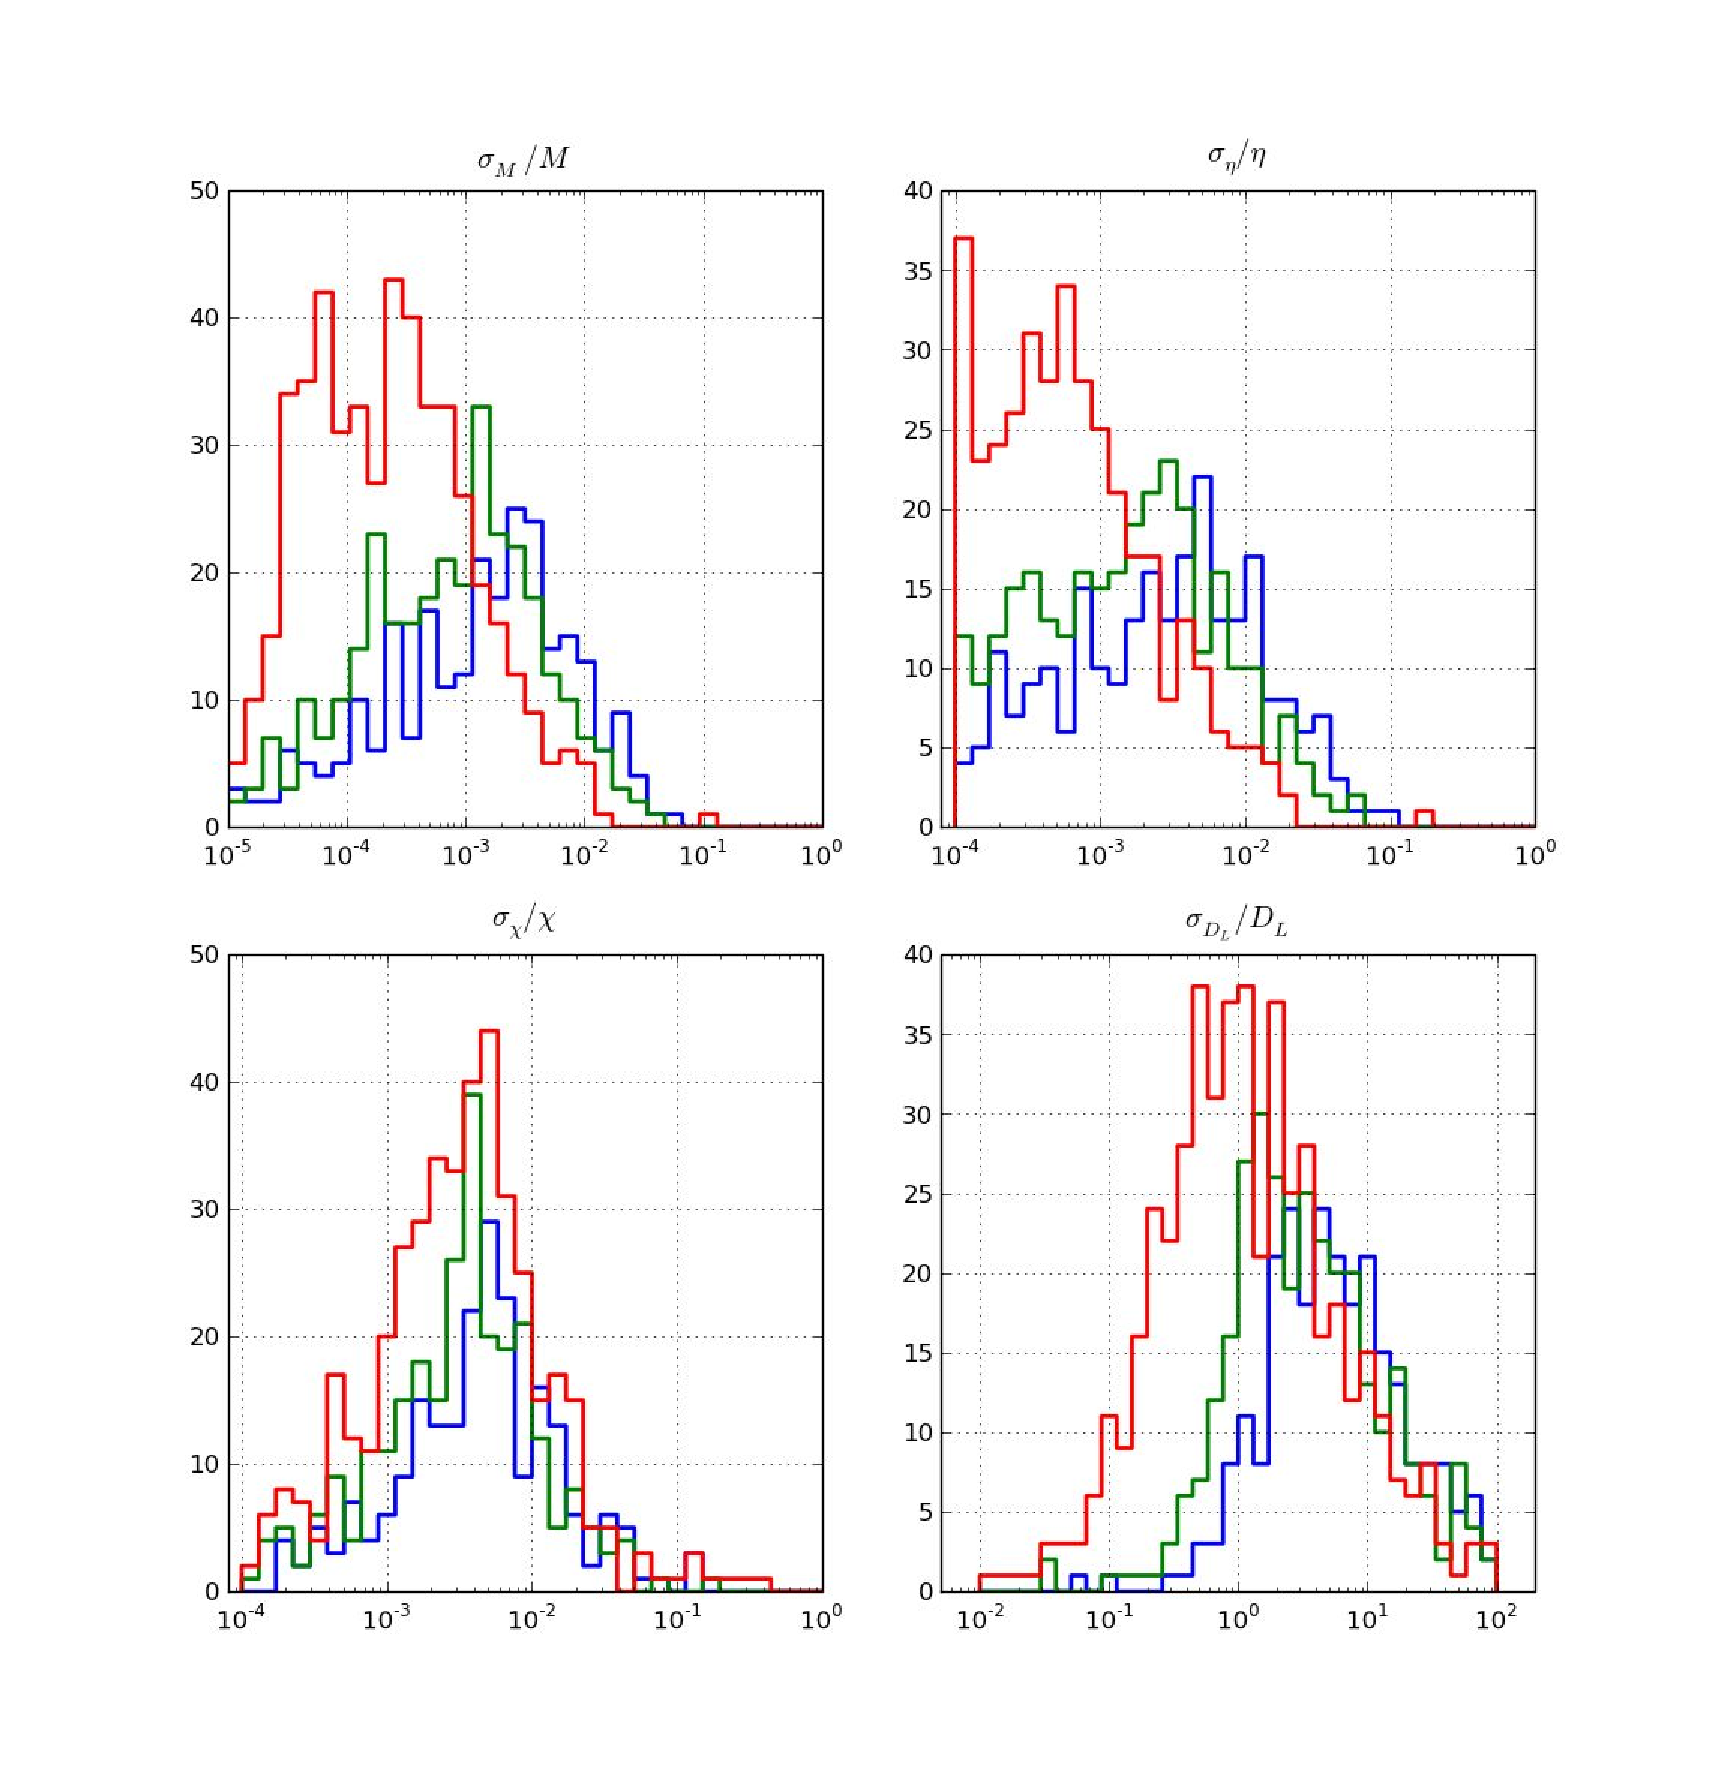
\includegraphics[scale=1,clip]{FigSMBHPhenomAEI/Hist_SE_LISAC1C2.eps}} 
\caption{1-$\sigma$ errors on source parameters: redshifted mass (upper left); symmetric mass ratio (upper right); spin parameter (lower left); luminosity distance (lower right). Histograms collect all the events in the SE catalogue, with SNR$>10$. Red histograms are for LISA, green histograms are for C2 and blue histograms are for C1.
\label{Hist_SE_LISAC1C2} } 
\end{figure}



\begin{figure}
\resizebox{\hsize}{!}{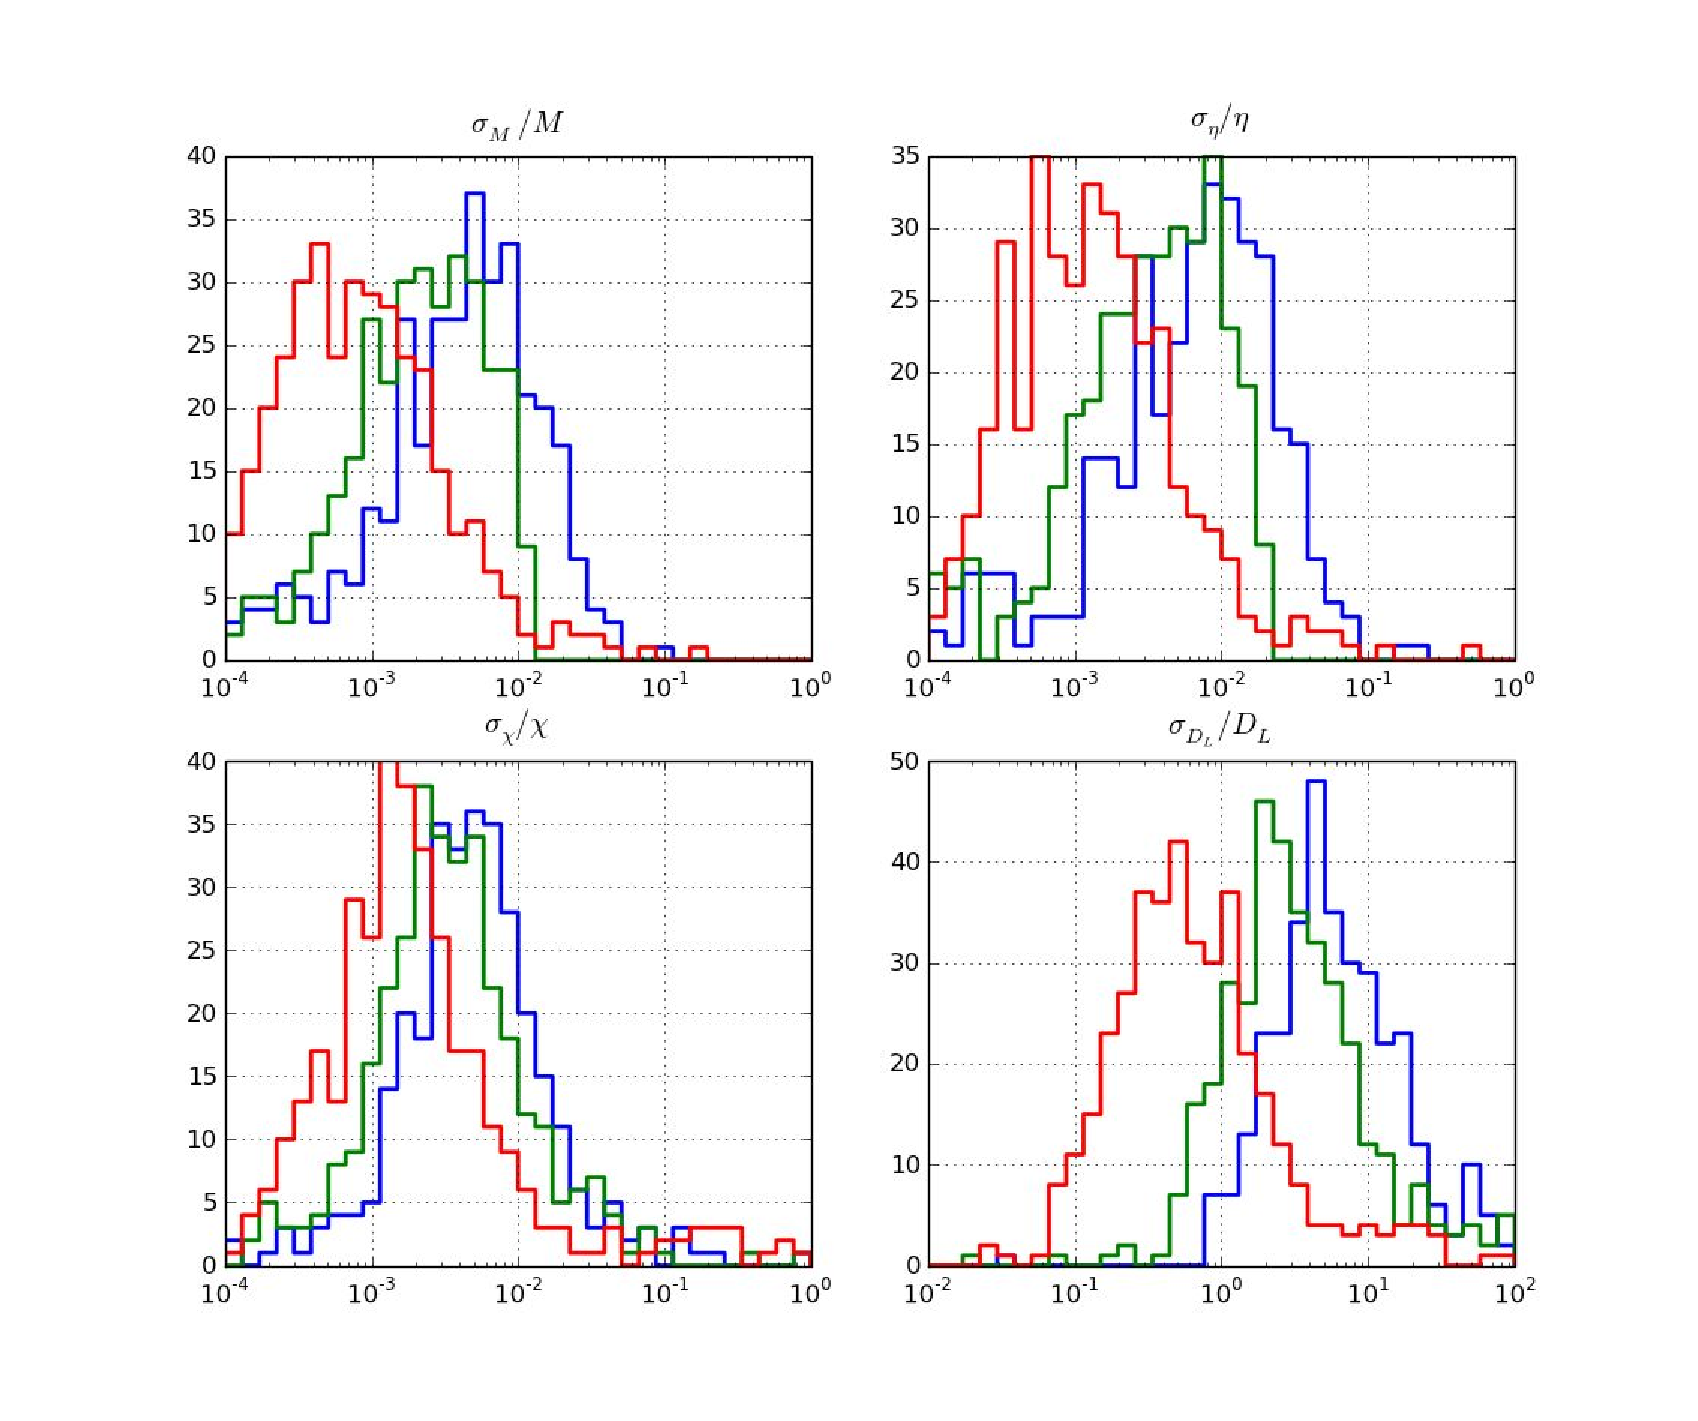
\includegraphics[scale=1,clip]{FigSMBHPhenomAEI/Hist_LE_LISAC1C2.eps}} 
\caption{Same as figure \ref{Hist_SE_LISAC1C2} but for the LE catalogue.
\label{Hist_LE_LISAC1C2} } 
\end{figure}


%%%%%%%%%%%%%%%%  Median erroe LISA, C1 and C3  %%%%%%%%%%%%%%%%


\begin{figure}
\resizebox{\hsize}{!}{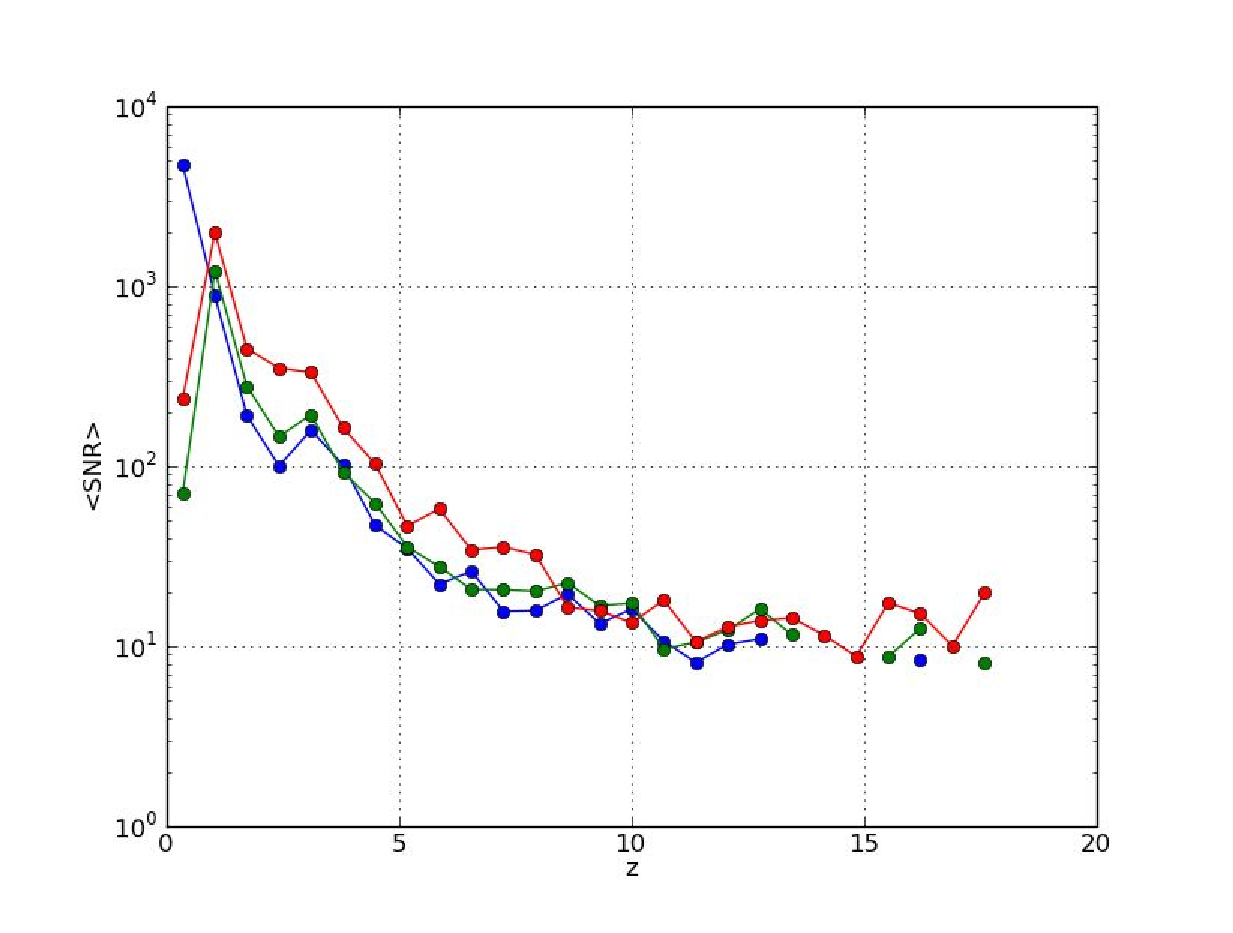
\includegraphics[scale=1,clip]{FigSMBHPhenomAEI/MedianSNR_SE_LISAC1C2.eps}} 
\caption{Median source SNR as a function of $z$. Colorstyle as in figure
\ref{Hist_SE_LISAC1C2}. Model SE is assumed.
\label{MedianSNR_SE_LISAC1C2} } 
\end{figure}



\begin{figure}
\resizebox{\hsize}{!}{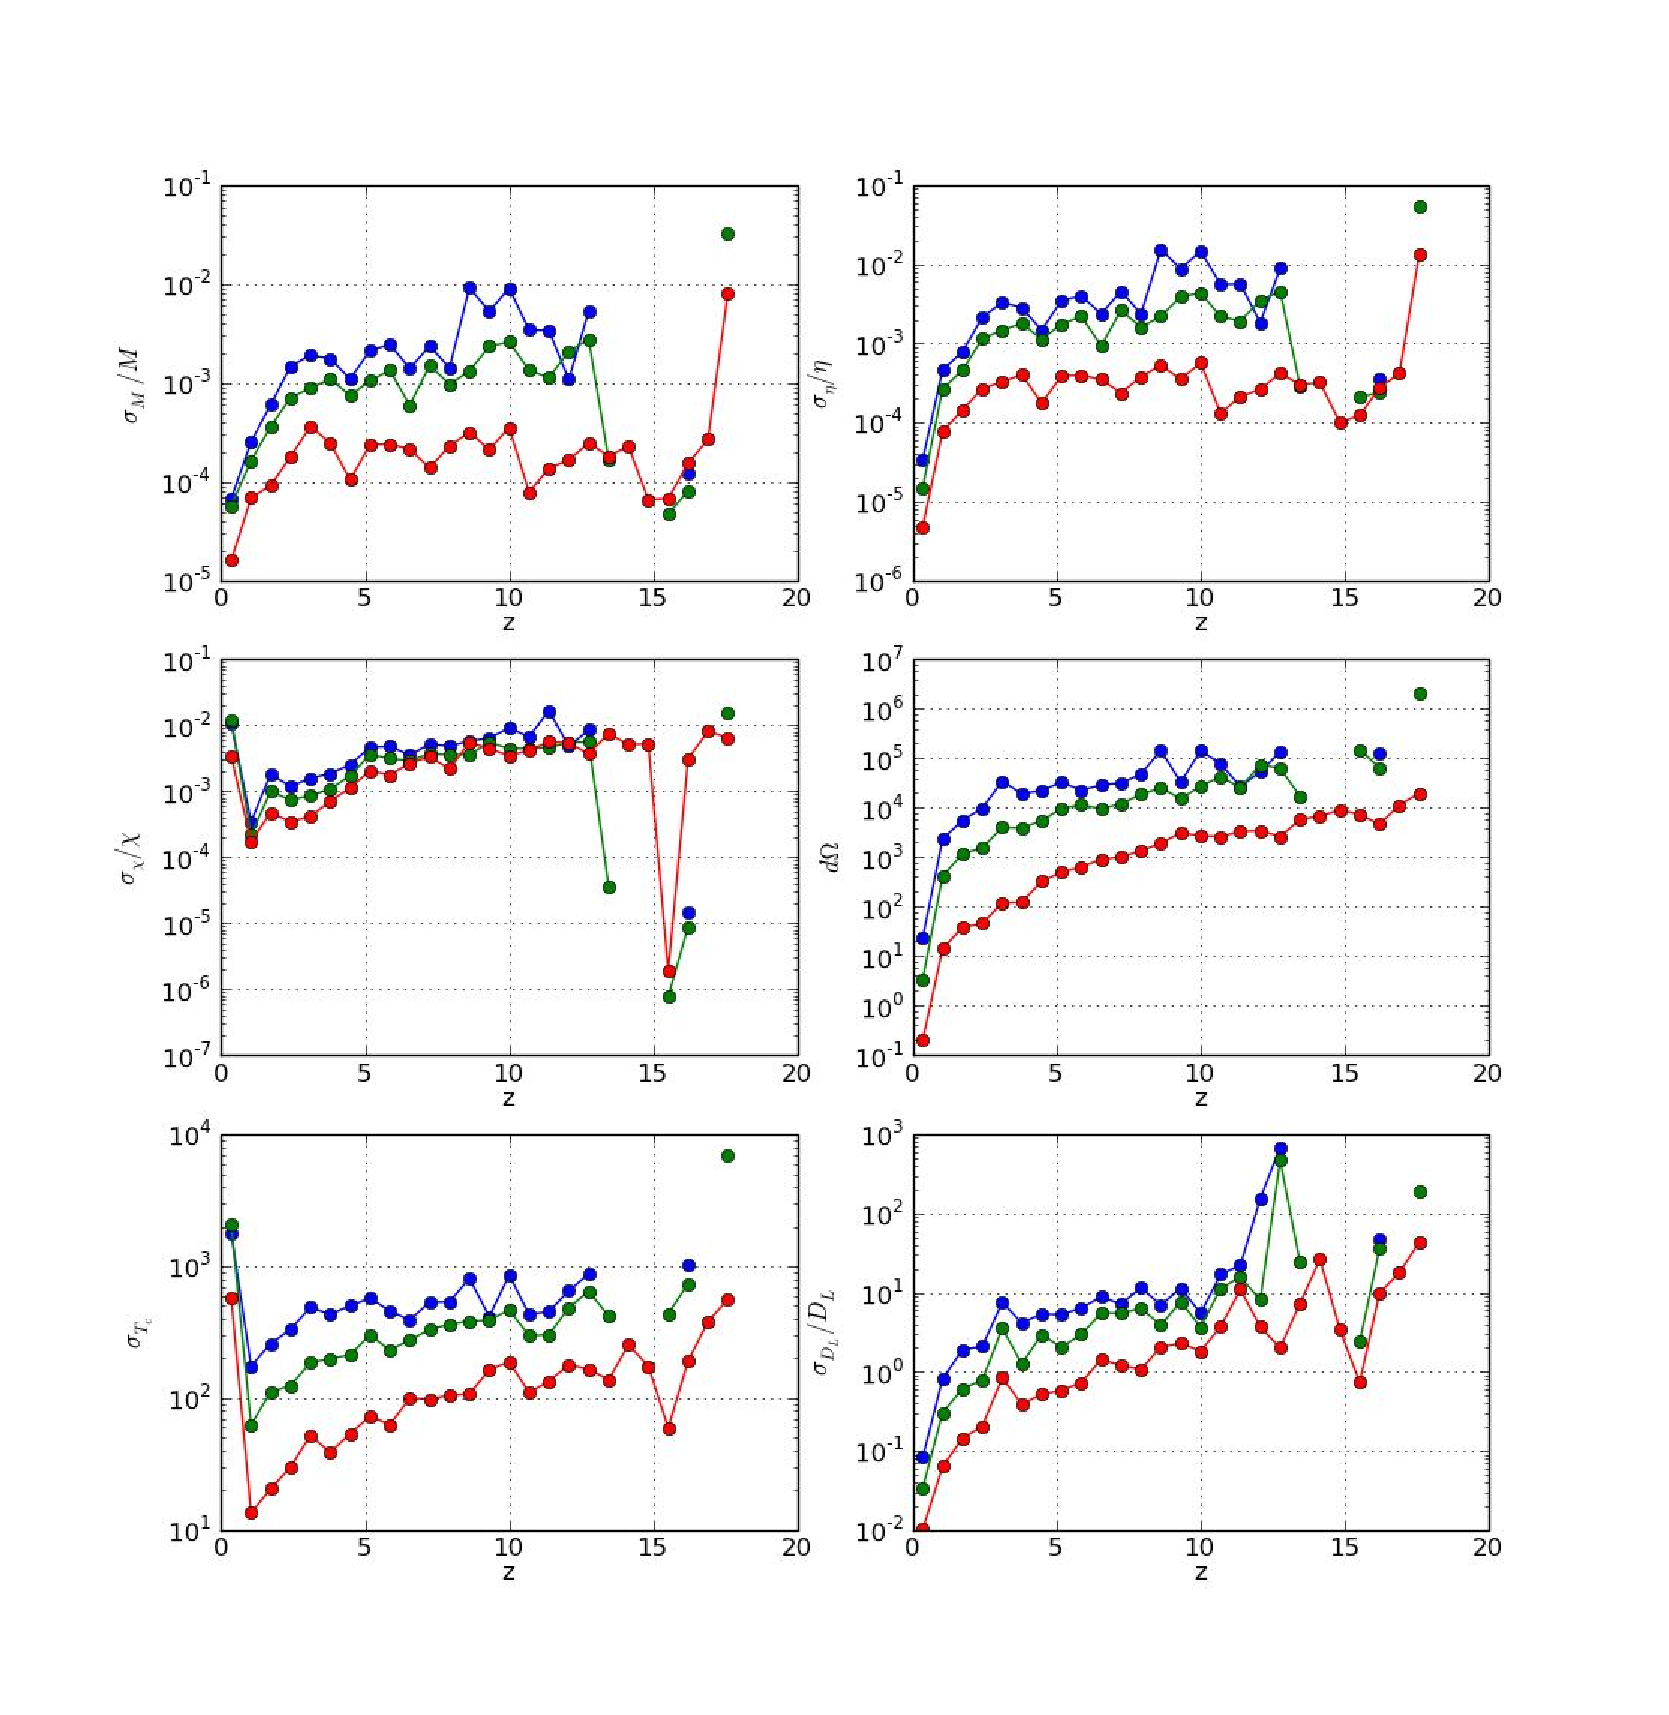
\includegraphics[scale=1,clip]{FigSMBHPhenomAEI/MedianErrs_SE_LISAC1C2.eps}} 
\caption{Median 1-$\sigma$ errors on the source parameters as a function of 
$z$: redshifted mass (upper left); symmetric mass ratio (upper right); spin parameter (middle left); sky location in deg$^2$ (middle right); coalescence time in seconds (lower left); luminosity distance (lower right). Colorstyle as in figure \ref{fig4}. Model SE is assumed.
\label{MedianErrs_SE_LISAC1C2} } 
\end{figure}



\begin{figure}
\resizebox{\hsize}{!}{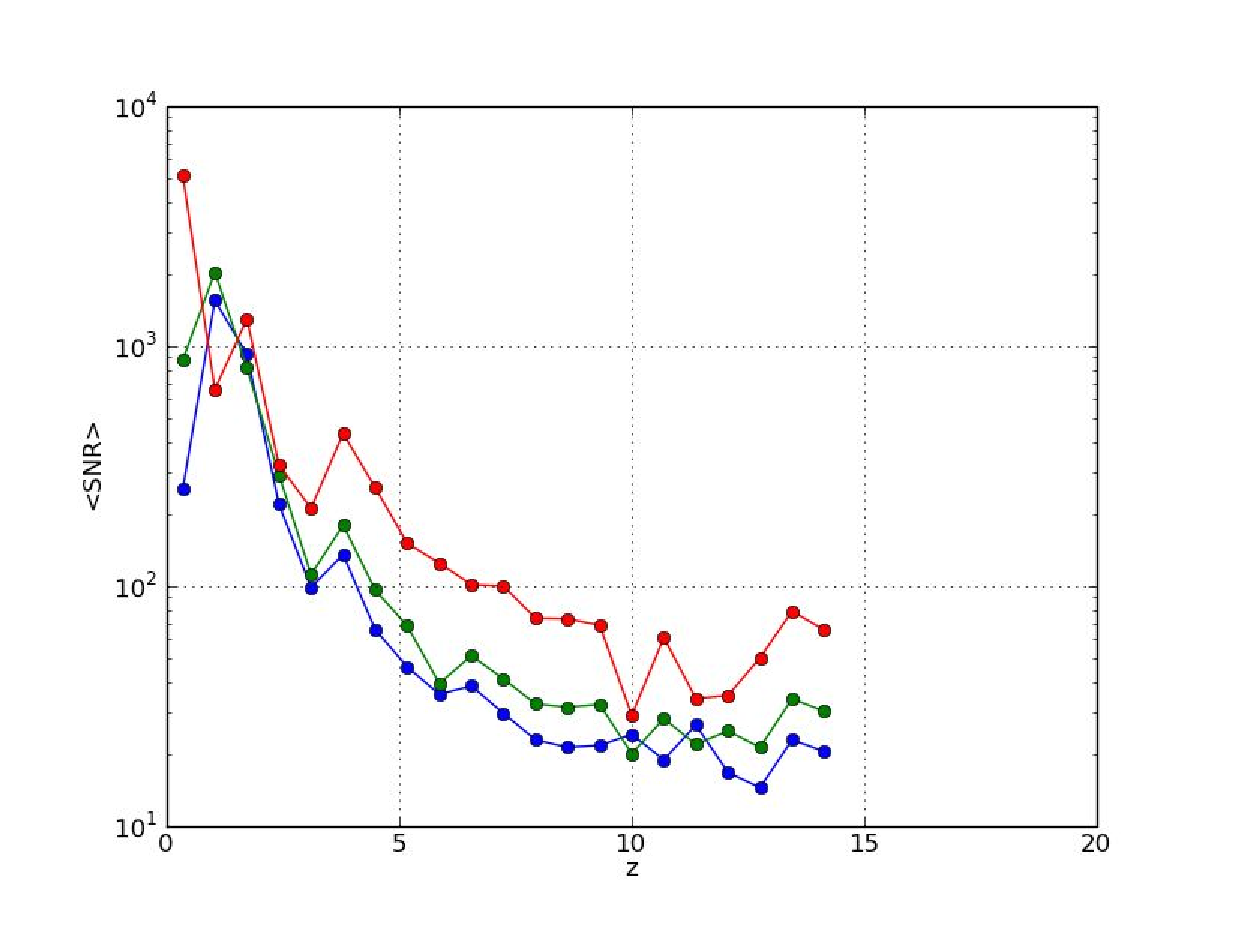
\includegraphics[scale=1,clip]{FigSMBHPhenomAEI/MedianSNR_LE_LISAC1C2}} 
\caption{Same as figure \ref{MedianErrs_SE_LISAC1C2} but for the LE catalogue.
\label{MedianSNR_LE_LISAC1C2} } 
\end{figure}



\begin{figure}
\resizebox{\hsize}{!}{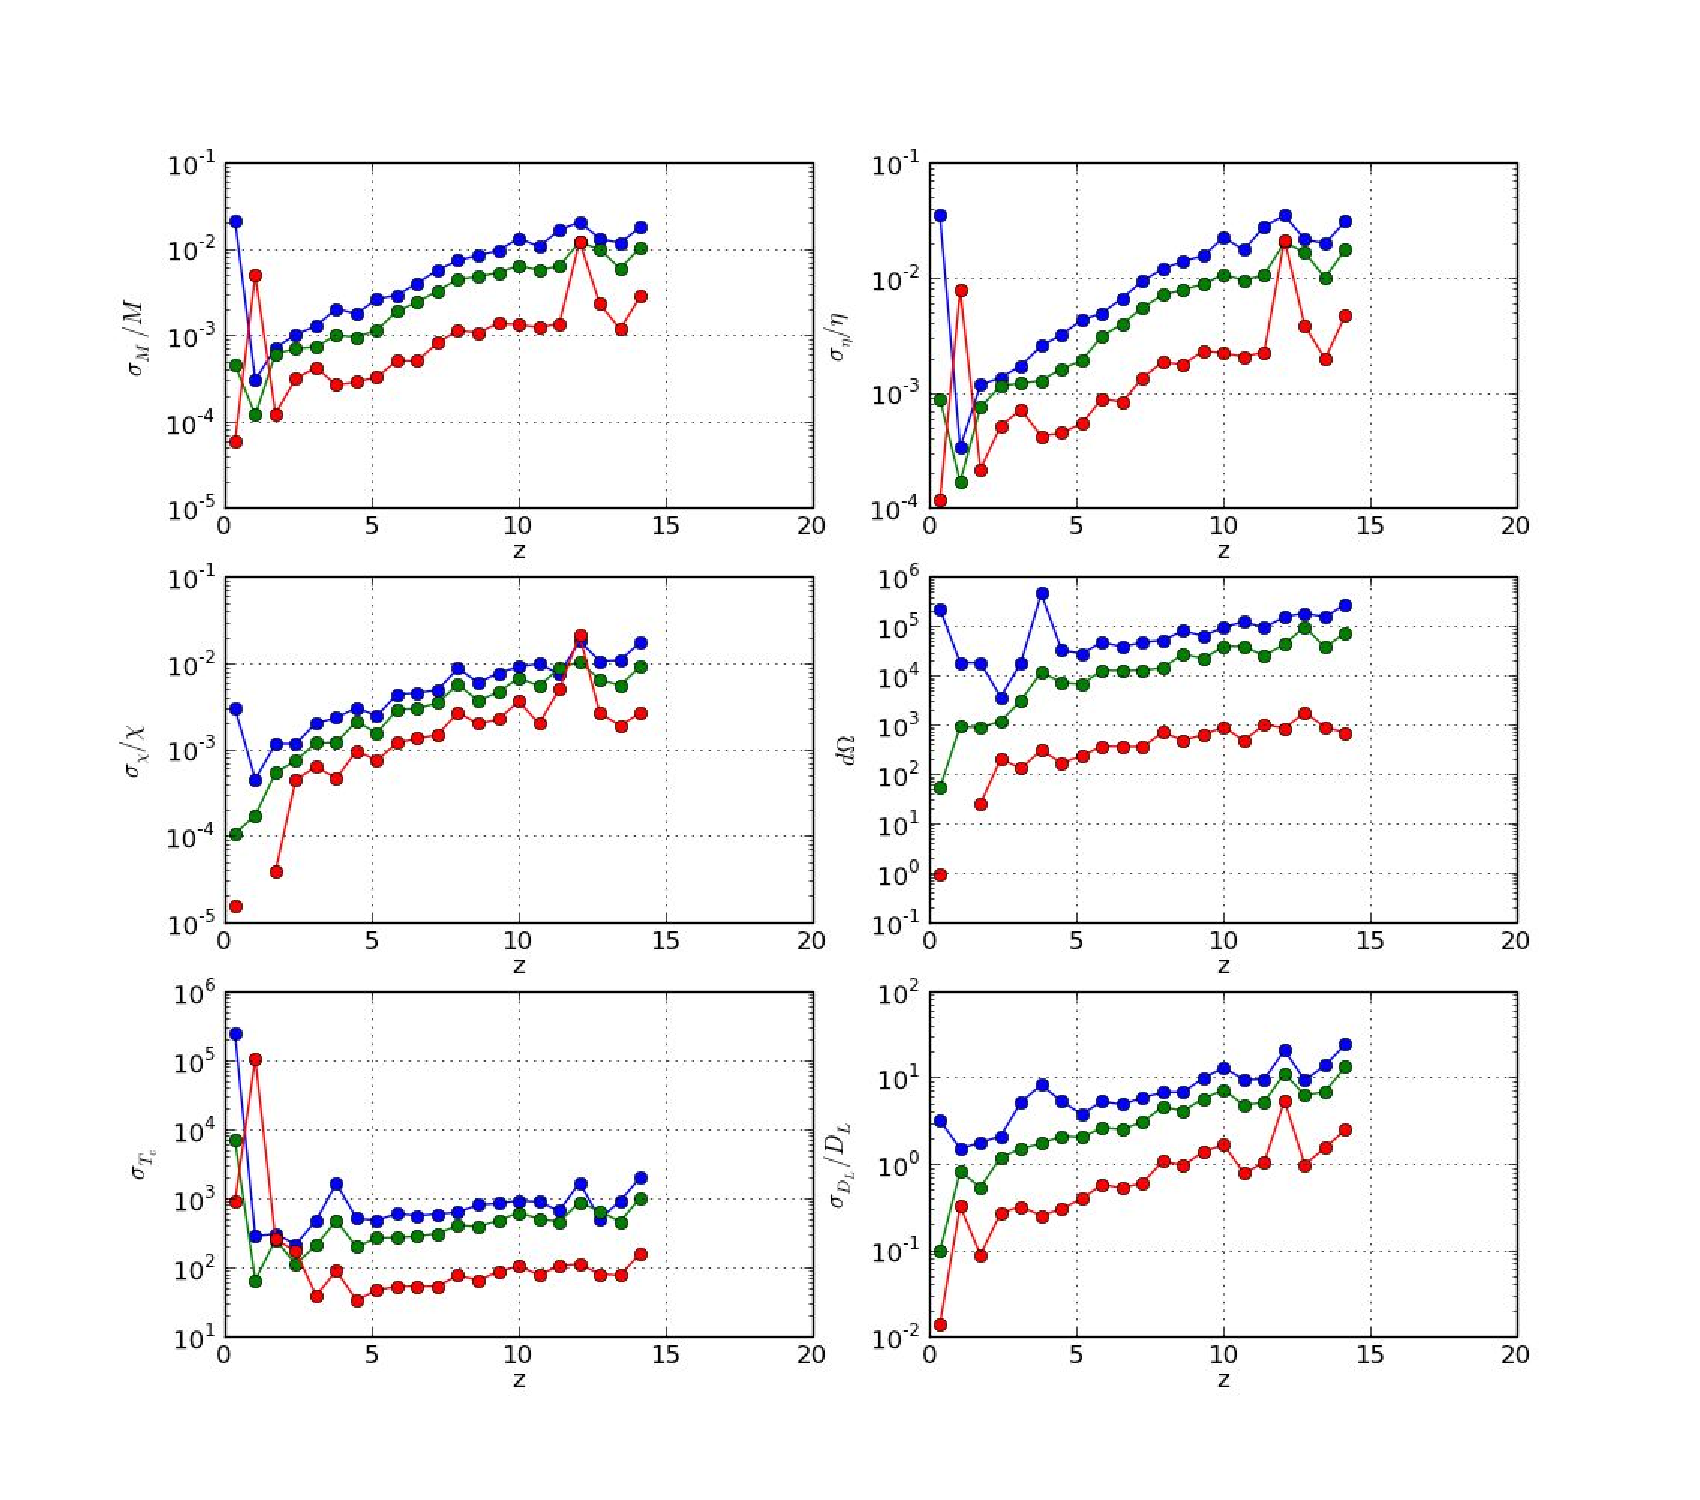
\includegraphics[scale=1,clip]{FigSMBHPhenomAEI/MedianErrs_LE_LISAC1C2}} 
\caption{Same as figure \ref{MedianErrs_SE_LISAC1C2} but for the LE catalogue.
\label{MedianErrs_LE_LISAC1C2} } 
\end{figure}















%%%%%%%%%%%%%%%    Model selection 
\subsection{Model selection}
\label{SS:MBHbModel}
{\it ('section captain' : Alberto Sesana) }
























%%%%%%%%%%%%%%%%%%%%%%%%%%%%%%%%%%%%%
%                                                            EMRIs                                                        %
%%%%%%%%%%%%%%%%%%%%%%%%%%%%%%%%%%%%%

\section{EMRIs}
{\it ('section captains' : Jon Gair \& Ed Porter) }

























\begin{thebibliography}{}

\bibitem{sm10}
L. Santamaria, F. Ohme, P. Ajith, B. Bruegmann, N. Dorband, M. Hannam, S. Husa, P. Moesta, D. Pollney, C. Reisswig, E. L. Robinson, J. Seiler and B. Krishnan,  Phys.\ Rev.\  D {\bf 82}, 064016 (2010)

\end{thebibliography}{}





\end{document}



